\documentclass[man]{apa6}
\usepackage{lmodern}
\usepackage{amssymb,amsmath}
\usepackage{ifxetex,ifluatex}
\usepackage{fixltx2e} % provides \textsubscript
\ifnum 0\ifxetex 1\fi\ifluatex 1\fi=0 % if pdftex
  \usepackage[T1]{fontenc}
  \usepackage[utf8]{inputenc}
\else % if luatex or xelatex
  \ifxetex
    \usepackage{mathspec}
  \else
    \usepackage{fontspec}
  \fi
  \defaultfontfeatures{Ligatures=TeX,Scale=MatchLowercase}
\fi
% use upquote if available, for straight quotes in verbatim environments
\IfFileExists{upquote.sty}{\usepackage{upquote}}{}
% use microtype if available
\IfFileExists{microtype.sty}{%
\usepackage{microtype}
\UseMicrotypeSet[protrusion]{basicmath} % disable protrusion for tt fonts
}{}
\usepackage{hyperref}
\hypersetup{unicode=true,
            pdftitle={The title},
            pdfkeywords={Rule-following behavior, partner choice, social environments},
            pdfborder={0 0 0},
            breaklinks=true}
\urlstyle{same}  % don't use monospace font for urls
\usepackage{color}
\usepackage{fancyvrb}
\newcommand{\VerbBar}{|}
\newcommand{\VERB}{\Verb[commandchars=\\\{\}]}
\DefineVerbatimEnvironment{Highlighting}{Verbatim}{commandchars=\\\{\}}
% Add ',fontsize=\small' for more characters per line
\usepackage{framed}
\definecolor{shadecolor}{RGB}{248,248,248}
\newenvironment{Shaded}{\begin{snugshade}}{\end{snugshade}}
\newcommand{\AlertTok}[1]{\textcolor[rgb]{0.94,0.16,0.16}{#1}}
\newcommand{\AnnotationTok}[1]{\textcolor[rgb]{0.56,0.35,0.01}{\textbf{\textit{#1}}}}
\newcommand{\AttributeTok}[1]{\textcolor[rgb]{0.77,0.63,0.00}{#1}}
\newcommand{\BaseNTok}[1]{\textcolor[rgb]{0.00,0.00,0.81}{#1}}
\newcommand{\BuiltInTok}[1]{#1}
\newcommand{\CharTok}[1]{\textcolor[rgb]{0.31,0.60,0.02}{#1}}
\newcommand{\CommentTok}[1]{\textcolor[rgb]{0.56,0.35,0.01}{\textit{#1}}}
\newcommand{\CommentVarTok}[1]{\textcolor[rgb]{0.56,0.35,0.01}{\textbf{\textit{#1}}}}
\newcommand{\ConstantTok}[1]{\textcolor[rgb]{0.00,0.00,0.00}{#1}}
\newcommand{\ControlFlowTok}[1]{\textcolor[rgb]{0.13,0.29,0.53}{\textbf{#1}}}
\newcommand{\DataTypeTok}[1]{\textcolor[rgb]{0.13,0.29,0.53}{#1}}
\newcommand{\DecValTok}[1]{\textcolor[rgb]{0.00,0.00,0.81}{#1}}
\newcommand{\DocumentationTok}[1]{\textcolor[rgb]{0.56,0.35,0.01}{\textbf{\textit{#1}}}}
\newcommand{\ErrorTok}[1]{\textcolor[rgb]{0.64,0.00,0.00}{\textbf{#1}}}
\newcommand{\ExtensionTok}[1]{#1}
\newcommand{\FloatTok}[1]{\textcolor[rgb]{0.00,0.00,0.81}{#1}}
\newcommand{\FunctionTok}[1]{\textcolor[rgb]{0.00,0.00,0.00}{#1}}
\newcommand{\ImportTok}[1]{#1}
\newcommand{\InformationTok}[1]{\textcolor[rgb]{0.56,0.35,0.01}{\textbf{\textit{#1}}}}
\newcommand{\KeywordTok}[1]{\textcolor[rgb]{0.13,0.29,0.53}{\textbf{#1}}}
\newcommand{\NormalTok}[1]{#1}
\newcommand{\OperatorTok}[1]{\textcolor[rgb]{0.81,0.36,0.00}{\textbf{#1}}}
\newcommand{\OtherTok}[1]{\textcolor[rgb]{0.56,0.35,0.01}{#1}}
\newcommand{\PreprocessorTok}[1]{\textcolor[rgb]{0.56,0.35,0.01}{\textit{#1}}}
\newcommand{\RegionMarkerTok}[1]{#1}
\newcommand{\SpecialCharTok}[1]{\textcolor[rgb]{0.00,0.00,0.00}{#1}}
\newcommand{\SpecialStringTok}[1]{\textcolor[rgb]{0.31,0.60,0.02}{#1}}
\newcommand{\StringTok}[1]{\textcolor[rgb]{0.31,0.60,0.02}{#1}}
\newcommand{\VariableTok}[1]{\textcolor[rgb]{0.00,0.00,0.00}{#1}}
\newcommand{\VerbatimStringTok}[1]{\textcolor[rgb]{0.31,0.60,0.02}{#1}}
\newcommand{\WarningTok}[1]{\textcolor[rgb]{0.56,0.35,0.01}{\textbf{\textit{#1}}}}
\usepackage{longtable,booktabs}
\usepackage{graphicx,grffile}
\makeatletter
\def\maxwidth{\ifdim\Gin@nat@width>\linewidth\linewidth\else\Gin@nat@width\fi}
\def\maxheight{\ifdim\Gin@nat@height>\textheight\textheight\else\Gin@nat@height\fi}
\makeatother
% Scale images if necessary, so that they will not overflow the page
% margins by default, and it is still possible to overwrite the defaults
% using explicit options in \includegraphics[width, height, ...]{}
\setkeys{Gin}{width=\maxwidth,height=\maxheight,keepaspectratio}
\IfFileExists{parskip.sty}{%
\usepackage{parskip}
}{% else
\setlength{\parindent}{0pt}
\setlength{\parskip}{6pt plus 2pt minus 1pt}
}
\setlength{\emergencystretch}{3em}  % prevent overfull lines
\providecommand{\tightlist}{%
  \setlength{\itemsep}{0pt}\setlength{\parskip}{0pt}}
\setcounter{secnumdepth}{0}
% Redefines (sub)paragraphs to behave more like sections
\ifx\paragraph\undefined\else
\let\oldparagraph\paragraph
\renewcommand{\paragraph}[1]{\oldparagraph{#1}\mbox{}}
\fi
\ifx\subparagraph\undefined\else
\let\oldsubparagraph\subparagraph
\renewcommand{\subparagraph}[1]{\oldsubparagraph{#1}\mbox{}}
\fi

%%% Use protect on footnotes to avoid problems with footnotes in titles
\let\rmarkdownfootnote\footnote%
\def\footnote{\protect\rmarkdownfootnote}

%%% Change title format to be more compact
\usepackage{titling}

% Create subtitle command for use in maketitle
\providecommand{\subtitle}[1]{
  \posttitle{
    \begin{center}\large#1\end{center}
    }
}

\setlength{\droptitle}{-2em}

  \title{The title}
    \pretitle{\vspace{\droptitle}\centering\huge}
  \posttitle{\par}
    \author{true \\ true}
    \preauthor{\centering\large\emph}
  \postauthor{\par}
    \date{}
    \predate{}\postdate{}
  

\begin{document}
\maketitle
\begin{abstract}
Abstract goes here.
\end{abstract}

\begin{Shaded}
\begin{Highlighting}[]
\CommentTok{# Seed for random number generation}
\KeywordTok{set.seed}\NormalTok{(}\DecValTok{42}\NormalTok{)}
\NormalTok{knitr}\OperatorTok{::}\NormalTok{opts_chunk}\OperatorTok{$}\KeywordTok{set}\NormalTok{(}\DataTypeTok{cache.extra =}\NormalTok{ knitr}\OperatorTok{::}\NormalTok{rand_seed)}
\end{Highlighting}
\end{Shaded}

Complex social norm systems are rules and standards that guide human
behavior in groups (Cialdini 2001; Pepitone 1976) and are unique to
human beings (Tomasello and Rakoczy 2003; Fehr and Rockenbach 2004;
Gintis 2003; Ostrom 2000; Sethi and Somanathan 1996; Fehr and
Fischbacher 2003). Importantly, abiding to social norms is generally
considered desirable as doing so is associated with good character
(Hoffman 1977; Freud 1977) which, in turn, helps building and
maintaining functioning societies. For example, policy makers and
legislators set guidelines and rules for societies that individuals
should adhere to and in response to such structures, rule-following
behavior then reflects moral character signaling trustworthiness
(Hoffman 1977; Freud 1977; Everett, Pizarro, and Crockett 2016; Baumard
et al. 2014).

Yet, people often choose to violate norms (Köbis et al. 2016) and engage
in corrupt collaborations (Weisel and Shalvi 2015) such as bribery
(Rose-Ackerman and Palifka 2016), trafficking (Nieto 2012), crime and
fraud (Ades and Tella 1996) by definition among many others. For
example, Mexico has been the center of drug violence, killing throusands
of people, and exposing the Mexican society to torture and impunity
(Nieto 2012). Also, the terrorist organization Islamic State in Iraq and
Syria (ISIS) caused numerous organized terrorist attacks across Europe
over the recent years (Farwell 2014). The consequences of such
corruption can be fatal including hindrance of economic growth (Mauro
1995) as well as undermined legitimacy and capacity of governments
(Rothstein 2011), hence, harming the functioning of societies. We
therefore need to determine under which circumstances people abide or
break rules.

Previous research highlighted the importance of interpersonal variables
in predicting cooperative behavior through morality goals. As people
like to think of themselves as moral beings (Mazar, Amir, and Ariely
2008; Jordan, Mullen, and Murnighan 2011; Abeler, Becker, and Falk 2014;
Abeler, Nosenzo, and Raymond 2019) and care about what others think of
them (Lacetera and Macis 2010; Utikal and Fischbacher 2013; Gausel and
Leach 2011), moral traits dominate (Cottrell, Neuberg, and Li 2007;
Landy and Uhlmann 2018; Landy, Piazza, and Goodwin 2016; Peeters 1992;
Wojciszke, Abele, and Baryla 2009). For example, besides traits such as
being sociable and warm (Goodwin 2015), people prefer to interact with
others who signal their trustworthiness (Hoffman 1977; Freud 1977)
because doing so signals being a `good' interaction partner.

Humans are social beings and when in groups, people prefer others they
can rely on, where cues of morality such as rule-following behavior are
a good indicator of this (Abele and Wojciszke 2014; Baumard et al. 2014;
Cottrell, Neuberg, and Li 2007; Landy, Piazza, and Goodwin 2016; Landy
and Uhlmann 2018; Peeters 1992; Wojciszke, Abele, and Baryla 2009). In
this regard, people typically perform costly behaviors that signal trust
(Jordan et al. 2016). For example, companies in the free market such as
Fairtrade and Tony's Chocolonely use logos with moral appeals to signal
their trustworthiness to both their customers and other companies, all
of which aim to facilitate cooperation. But companies do not often
function in isolation, rather in a market with competitors and partners,
and it is this competition that can make companies and individuals more
cooperative. For example, Barclay and Willer (2006) found that when
people have the opportunity to be selected as a partner and benefit from
this interaction, people competed against others to signal they were
more generous than their competitors. The most generous therefore
signaled being better interaction partners than others as an indicator
of moral character. Biological markets and the pressures that arise
along with them can therefore facilitate cooperation.

The effects of partner choice have mainly been investigated in
cooperation settings using economic games, where providing people with
the freedom to seek out trustworthy partners and abandon free-riders has
been shown to develop and safeguard cooperation (Efferson et al. 2016;
Rand, Arbesman, and Christakis 2011). Therefore, cooperation is usually
more lucrative than defection. For example, in hunter-gatherer networks,
those who share their spoils form more profitable relationships than
those who do not (Gurven et al. 2000). Also, the European Union (EU) and
the United Nations (UN) represent international alliances where nations
collaborate with each other. However, which agents are chosen as
interaction partners, depends on how able and inclined these agents are
to benefit others (Barclay 2013; André and Baumard 2011; Baumard, André,
and Sperber 2013). Benefits can take on the form of wealth, mutual gain,
talents, and resources (Hirschman 1987; Montesquieu 1951).

Yet, in other settings, people choose to be corrupt as a collective,
where corrupt collaboration is defined as attaining personal profits as
the result of joint acts of rule violations (Weisel and Shalvi 2015),
and depends on the omral goals people have (Everett, Pizarro, and
Crockett 2016; Baumard et al. 2014) and the context people are in
(Melnikoff and Bailey 2018). Example for such corruption is the
Volkswagen scandal from 2005 where the employees of the company
manipulated software to pass key emission tests in the face of limited
time and budget and hence likely personal benefits (Goodman 2015).
However, as if corrupt collaboration itself was not enough, corruption
breeds corruption. For example, countries that are plagued by more
corruption have been found to have a higher black market premium
(Bahmani-Oskooee and Goswami 2005), and higher inflation rates
(Cukierman, Edwards, and Tabellini 1989), all of which go at the expense
of the poor (Gupta, Davoodi, and Alonso-Terme 1998). As these examples
demonstrate, we have to research the determinants that benefit societies
and those that destroy them.

\hypertarget{the-present-experiment}{%
\section{The present experiment}\label{the-present-experiment}}

We argue that a) divergent selective pressures of the social
environments people are in determine behaviors that signal `being a good
partner' and that b) cooperation is not prosocial per se but critically
depends on both the social environment and having the mere option to
choose one's social interaction partners.

\emph{Hypothesis 1}: Norms of rule-following behavior will establish
specific to the two settings. Specifically, over time, we expect
rule-following scores to decrease in the corrupt environment (H1a) and
to increase in the prosocial environment (H1b).

\emph{Hypothesis 2}: Across environments, rule-following behavior is
anchored in setting A and modifies the trend in environment B.
Specifically, we expect that if the corrupt environment is shown second,
the trend of rule-following scores will decline but less than if the
corrupt environment is shown first (H2a). Also, we expect that if the
prosocial environment is shown second, the reverse will occur (H2b).

\emph{Hypothesis 3}: In a biological market, partner choice shapes
rule-following behavior. Specifically, we expect that in the corrupt
environment, those with a low rule-following score will be selected more
than those with a high score. We expect the reverse in the prosocial
environment.

To test these hypotheses, we conducted an experiment with a series of
game-theoretic tasks in one experimental session lasting one hour.

\hypertarget{how-moral-to-be}{%
\subsection{How moral to be}\label{how-moral-to-be}}

\hypertarget{what-partners-to-choose}{%
\subsection{What partners to choose}\label{what-partners-to-choose}}

Behavior that is costly to perform signals trust, a moral trait and
fundamental building block of relationships.

Costly signaling theory holds that behaviors can be costly to perform
but entail trust in return - regardless of whether these behaviors are
intended or unintended {[}ref{]}.

\hypertarget{when-we-cooperate}{%
\subsection{When we cooperate}\label{when-we-cooperate}}

The effects of partner choice have mainly been investigated in
cooperation settings using economic games like the Prisoner's dilemma
game, which allow for analysing the evolution of cooperation and the
establishment of nomative behavior.

Indeed, effects of partner choice have mainly been investigated in
cooperation settings and have been shown to \ldots{} to structure social
preferences, make reputation concerns more salient, \ldots{}

\hypertarget{when-we-corrupt-and}{%
\subsection{When we corrupt and}\label{when-we-corrupt-and}}

\hypertarget{methods}{%
\section{Methods}\label{methods}}

We report how we determined our sample size, all data exclusions, all
manipulations, and all measures in the study (Simmons, Nelson, and
Simonsohn 2012).

\hypertarget{participants-and-ethics}{%
\subsection{Participants and ethics}\label{participants-and-ethics}}

Participants were recruited from the subjects pool of the Faculty of
Social and Behavioural Sciences at Leiden University. Each of the 212
participants consented digitally to take part in one experimental
session lasting approximately one hour and were debriefed digitally.
Zero participants withdrew their participation. 12 participants were
excluded due to server overload and resulting incomplete data.
Therefore, the data of 200 participants was used for our analyses.
Participants (mean age = 23.06 +/− 4.25, 155 female) were paid €9,08 on
average. The experimental tasks were programmed using oTree (Chen,
Schonger, and Wickens 2016).Screenshots of the instructions are appended
to the Supplemental Material and all data and materials are available on
OSF (\url{https://osf.io/v4rma/}).

\hypertarget{experimental-design-and-setup}{%
\subsection{Experimental design and
setup}\label{experimental-design-and-setup}}

We conducted an interactive group experiment involving a series of
game-theoretic tasks. Figure {[}x{]} summarises both the timeline and
the experimental tasks. We used one between-subjects factor (role:
selector vs decider) and one within-subjects factor (setting: trust vs
dishonesty). In all experimental sessions, four participants were
randomly grouped together depending on their availabilities. Over a
total of 30 rounds, participants went through a sequence of three stages
in each round: a rule-following tasks (stage one), a partner selection
task (stage two), and two settings - a trust game and a dyadic
die-rolling task - for 15 rounds each (stage three). All participants
were exposed to both settings and went through different stages based
their role and the decisions others made. After the experimental blocks,
all participants did the die-rolling task by themselves and filled in
the social value orientation (SVO) scale, their demographics, and
answered control questions.

The currency in the experiment was points, where 100 points = €1.00.
Participants accumulated their points individually based on their
choices and over the three stages. Earnings could range from €6.50 to
€14.50. Alternatively, participants could get paid out 2 SONA credits
plus the bonus. If they collected less than 650 points, they were paid
the show-up fee of €6.50. However, if they collected more than 650
points, all exceeding points were considered their bonus. To calculate
the participants' final payment, two rounds of the total 30 were
randomly selected by the computer. The total summed amount of points
they collected in these two rounds plus the points from the last
die-roll task were converted to Euros and paid out to the participants.

\hypertarget{experimental-procedure}{%
\subsection{Experimental procedure}\label{experimental-procedure}}

Participants typically arrived separately at the laboratory and were
seated in individual cubicles with computers. At the end of the
experiment, they were asked to remain seated inside the cubicles and
wait for an experimenter to open the door. We informed the participants
that the present study was a group experiment in which they would
interact with other participants in a group of four in total. They were
also told how many of the group members already arrived and how many
were still missing. We stressed this to make sure they trusted their own
decisions to have an impact on other real human individuals.
Participants were told that the entire experiment was computerised. The
consent and debriefing forms were therefore shown on the computers. This
study fell under the no-deception policy of Leiden University. So, there
were neither hidden information nor deception in the study, and
everything was done as stated in the instructions. After completing the
comprehension checks, participants went on to the first task.

\hypertarget{stage-one-the-rule-following-task}{%
\subsubsection{Stage One: the rule-following
task}\label{stage-one-the-rule-following-task}}

The key variable of interest was rule-following behaviour. Participants
were presented with 15 balls they could allocate one-by-one to either a
blue or a yellow bucket (by clicking with the cursor on the buckets'
respective buttons on the computer screen). Participants were instructed
that `the rule is to put the balls in the blue bucket'. They had no
reason for following the rule and did not face any consequences if they
did not. The rule-following variable was operationalized as a score of
the summed number of balls put in the blue bucket per round and could
range from 0 to 15. Instructions read that each ball put in the blue
bucket would earn them 5 points and that each ball put in the yellow
bucket would earn them 15 points. So, choosing to put all balls in the
blue bucket earned participants only a third (75 points) of what they
could have earned if they put all balls in the yellow bucket (225
points). A counter below the buckets' buttons showed the amount of money
they accumulated (Kimbrough and Vostroknutov 2016). Participants
received feedback about the scores of the other group members. To avoid
reputation concerns, in all stages, feedback displays were sorted by the
highest rule-following score (i.e.~the summed number of balls put in the
blue bucket) in descending order. At the end of each round,
rule-following scores were reset to 0 to avoid reputation effects
(Milinski, Semmann, and Krambeck 2002).

\begin{itemize}
\tightlist
\item
  reasoning for incentive scheme: why those numbers?
\end{itemize}

\hypertarget{stage-two-partner-selection}{%
\subsubsection{Stage Two: partner
selection}\label{stage-two-partner-selection}}

The partner selection variable was the number of partners selected per
round. Participants were randomly assigned to one of two roles: selector
or decider. One of the four group members was in the selector role, the
other three were in the decider role. Selectors skipped the
rule-following task. However, in the second stage, selectors had to
select at least one of the deciders - but could also choose two or even
all three deciders - for the third stage. We excluded the possibility to
select zero deciders to avoid punishment effects (Fehr and Gächter
2002). All group members were informed that the selector had to spend
150 points for each selected decider. When selecting participants,
selectors received feedback about all deciders' rule-following scores.
In the meantime, deciders had to wait. If they got selected, they had to
decide about both their own and the selectors' earnings in the third
stage. Therefore, partners (i.e.~selected deciders) inevitably earned
more than those who were not and it was desirable to get selected.
Importantly, partners interacted with the selector only, not with the
other partners. Feedback about the selectors' decisions was provided to
all deciders and the feedback showed both the rule-following scores and
who got chosen. We expected participants to learn from the feedback
about who got chosen and who did not and adjust their choices in the
next round. Participants who got chosen continued to stage three and
participants who did not waited until the next round.

The partner selection variable was the number of partners selected per
round. Participants were randomly assigned to one of two roles: selector
or decider. Only one of the four group members was in the selector role,
the other three were in the decider role. Selectors skipped the
rule-following task. Instead, their role consisted on selecting at least
one of the deciders - they could also choose two or all three deciders -
for the third stage. Before allocating the balls to either bucket, all
group members were informed that there would be a selector, who had to
spend 150 points for each selected decider. When selecting participants,
selectors received feedback about all deciders' rule-following scores.
In the meantime, deciders had to wait. If they got selected, they had to
decide about both their own and the selectors' earnings in the third
stage. Therefore, partners (i.e.~selected deciders) inevitably earned
more than those who were not, and thus, it was desirable to get
selected. Importantly, partners interacted with the selector only, not
with the other partners. Feedback about the selectors' decisions was
provided to all deciders and the feedback showed both the rule-following
scores and who got chosen. We expected participants to learn from the
feedback about who got chosen and who did not and adjust their choices
in the next round. Participants who got chosen as interaction partners
continued to stage three and participants who did not, waited until the
next round.

\hypertarget{stage-three-two-settings}{%
\subsubsection{Stage Three: two
settings}\label{stage-three-two-settings}}

There were two settings in the third stage: a dictator game and a dyadic
die-rolling game. Each setting was repeated for 15 rounds and which one
was shown first depended on the condition of the particular sessions.
Therefore, the order of the settings was experimentally counterbalanced.

In one setting, participants played a modified dictator game in which
selectors could not reject the offer made by the individual partners
(i.e.~selected deciders). Therefore, punishment could not act as a
confound. In the game, the variable of interest was fairness and it was
conceptualised as the amount of points that partners gave to the
selectors. Partners were endowed with 500 points and had to allocate x
to the selector and kept 500 - x for themselves, where x could assume a
value between 0 and 250 in steps of 50 points. Options were shown in a
dropdown menu. Choosing the maximum of x = 250 resulted in a fair mutual
outcome and choosing the minimum of x = 0 resulted in a selfish outcome.
In this stage, selectors' earned totals were the sums of their partners'
allocated points, so that sum(1 to i) (500 - xi). Selectors received
feedback about all partners' allocations along with their rule-following
scores from the first stage. Then, the next round started.

In the other setting, partners played a modified version of the commonly
used dyadic die-rolling game (Weisel and Shalvi 2015; Fischbacher and
Föllmi-Heusi 2013; for a meta-analysis, see Abeler, Nosenzo, and Raymond
2019). Instead of two participants having to match their responses, only
the partners had to report a die-roll. The reported number determined
partners' own earnings and those of the selectors. The variable of
interest was dishonesty and the incentives for the die-rolling game were
set in such a way that participants had to be dishonest and coordinate
their reported die-roll outcomes with their partners if they wanted to
receive a relatively reasonable amount of points for themselves. Weisel
and Shalvi (2015) already observed people to coordinately report
die-roll outcomes and report a `double' 82\% of the time, a result that
exceeds chance (2.78\% for two separate die rolls with the same outcome)
and outcomes reported when alone. Both the partners and selectors earned
the same amount of points for the reported die roll, so that both earned
x points. Earnings ranged from 0 points (for reporting a 1) to 250
points (for reporting a 6) in steps of 50 points. For example, if a
partner reported a 4, the partner and selector both earned 150 points.
However, if a partner reported a 5, both earned 200 points. At the end
of every round, selectors received feedback about all partners'
contributions along with their rule-following score from the first
stage. Earnings of a selector were the sum of points that each of their
partners decided on or reported, so that sum(1 to i) (500 - xi). In
addition, all participants received feedback about their own earnings at
the end of each round. Then, the next round started. When participants
reached the end of round 30, they finished the experimental block and
continued to final individual-level measures.

\hypertarget{final-measures}{%
\subsubsection{Final measures}\label{final-measures}}

We measured a few potential individual-level confounds. First,
dishonesty could have had an influence on both the deciders' as well as
the selectors' decisions. Similar to the previous dyadic die-roll task,
this time, participants did a die-roll. However, this time, they did the
die-roll for themselves only. Hence, the die-roll only increased
participants' own earnings, not the earnings of any other group members.
Second, participants' concern for others could have affected their
decisions. We used a 6-item social value orientation (SVO) scale
(Murphy, Ackermann, and Handgraaf 2011) slider variant with continuous
choices. Last, we asked control questions about participants' motives to
participate, previous experiences with similar experiments, knowledge of
this experiment prior to its start, and whether they believed they
interacted with real human individuals. At the end of the experiment,
participants were debriefed and informed about their final earnings
digitally. They waited for an experimenter, got paid, and were thanked
for their participation.

\hypertarget{results}{%
\section{Results}\label{results}}

After checking the dataset for missing data and outliers, we will
analyze the diverging effects of the two settings (H1; the dictator game
and the die-rolling task) and their order (H2) on rule-following scores,
respectively. Then, we will test whether diverging partner choice
pressures arise in the two settings (H3).

First, there was no missing data and boxplots revealed no present
outliers, so that there were no observations with high leverage. We used
R (Version 3.5.1; R Core Team 2018) and the R-packages \emph{dplyr}
(Version 0.8.1; Wickham et al. 2019), \emph{DT} (Version 0.7; Xie,
Cheng, and Tan 2019), \emph{ggplot2} (Version 3.1.1; Wickham 2016),
\emph{gridExtra} (Version 2.3; Auguie 2017), \emph{knitr} (Version 1.23;
Xie 2015), \emph{lme4} (Version 1.1.21; Bates et al. 2015),
\emph{Matrix} (Version 1.2.14; Bates and Maechler 2018), \emph{papaja}
(Version 0.1.0.9842; Aust and Barth 2018), \emph{plyr} (Version 1.8.4;
Wickham et al. 2019; Wickham 2011), and \emph{xtable} (Version 1.8.3;
Dahl et al. 2018) for all our analyses. Our data is nested in groups and
therefore we can use a multilevel model with restricted maximum
likelihood (REML) taking the intraclass correlations into account
(Gelman and Hill 2006). To avoid multiply testing our dependent variable
(i.e., rule-following scores), we only use one unifying random
intercepts regression model for all hypotheses. The mathematical model
is specified in the Appendix.

\hypertarget{h1-establishing-norms-of-rule-following-behavior}{%
\subsection{H1: Establishing Norms of Rule Following
Behavior}\label{h1-establishing-norms-of-rule-following-behavior}}

Incentive structures of social settings determine behavior in groups. In
a corrupt setting, for example, people may abandon rules but in a
prosocial setting, people may do the opposite and adhere to rules
instead. However, will such behavioral tendencies toward rules establish
in our experiment? And more importantly, will norms of these tendencies
establish over time?

In line with our expectation, norms of rule following were established
in both settings as shown in Figure 1. However, to our surprise,
rule-following scores generally decreased over time (\emph{b} = -0.03,
95\% CI{[}-0.06;-0.00{]}) and did not change as a function of the
setting alone (\emph{b} = -0.20, 95\% CI{[}-1.11;0.70{]}). However, when
testing the interaction term between setting and round, rule-following
scores decreased in the corrupt setting more depending on the time
passed by (\emph{b} = -0.07, 95\% CI{[}-0.12;-0.01{]}). Interestingly,
as Figure 1 shows, both variables setting and round do not interact in
the first half (\emph{b} = -0.04, 95\% CI{[}-0.12;-0.04{]}), only in the
second (\emph{b} = -0.08, 95\% CI{[}-0.15;-0.02{]}). The main effect of
rounds on rule-following scores remains consistent across the halves
with the effect being stronger in the first half (\emph{b} = -0.17, 95\%
CI{[}-0.22;-0.11{]}) than the second (\emph{b} = -0.07, 95\%
CI{[}-0.12;-0.03{]}). Further differences between the halves may exist
and the order of the settings may play a vital role.

{[}Why?{]}

\begin{Shaded}
\begin{Highlighting}[]
\KeywordTok{setwd}\NormalTok{(}\StringTok{'/Users/sese/Desktop/Data/'}\NormalTok{)}
\NormalTok{result <-}\StringTok{ }\KeywordTok{read.table}\NormalTok{(}\StringTok{'result.csv'}\NormalTok{, }\DataTypeTok{header=}\NormalTok{T, }\DataTypeTok{sep=}\StringTok{','}\NormalTok{)}
\NormalTok{result <-}\StringTok{ }\NormalTok{result[,}\DecValTok{2}\OperatorTok{:}\KeywordTok{dim}\NormalTok{(result)[}\DecValTok{2}\NormalTok{]]}

\KeywordTok{library}\NormalTok{(ggplot2)}
\end{Highlighting}
\end{Shaded}

\begin{verbatim}
## Warning: package 'ggplot2' was built under R version 3.5.2
\end{verbatim}

\begin{Shaded}
\begin{Highlighting}[]
\NormalTok{apatheme=}\KeywordTok{theme_bw}\NormalTok{()}\OperatorTok{+}
\StringTok{  }\KeywordTok{theme}\NormalTok{(}\DataTypeTok{panel.grid.major=}\KeywordTok{element_blank}\NormalTok{(),}
        \DataTypeTok{panel.grid.minor=}\KeywordTok{element_blank}\NormalTok{(),}
        \DataTypeTok{panel.border=}\KeywordTok{element_blank}\NormalTok{(),}
        \DataTypeTok{axis.line=}\KeywordTok{element_line}\NormalTok{(),}
        \DataTypeTok{text=}\KeywordTok{element_text}\NormalTok{(}\DataTypeTok{family=}\StringTok{'serif'}\NormalTok{, }\DataTypeTok{size =} \DecValTok{15}\NormalTok{),}
        \DataTypeTok{legend.text =} \KeywordTok{element_text}\NormalTok{(}\DataTypeTok{family =} \StringTok{'serif'}\NormalTok{, }\DataTypeTok{size =} \DecValTok{15}\NormalTok{),}
        \DataTypeTok{axis.text =} \KeywordTok{element_text}\NormalTok{(}\DataTypeTok{family =} \StringTok{'serif'}\NormalTok{, }\DataTypeTok{size =} \DecValTok{15}\NormalTok{, }\DataTypeTok{colour =} \StringTok{'black'}\NormalTok{),}
        \DataTypeTok{legend.title=}\KeywordTok{element_blank}\NormalTok{(),}
        \DataTypeTok{plot.caption =} \KeywordTok{element_text}\NormalTok{(}\DataTypeTok{hjust =} \FloatTok{0.05}\NormalTok{, }\DataTypeTok{family =} \StringTok{'serif'}\NormalTok{, }\DataTypeTok{size =} \DecValTok{15}\NormalTok{)) }


\CommentTok{# h1}

\NormalTok{half1 <-}\StringTok{ }\DecValTok{1}\OperatorTok{:}\DecValTok{15}
\NormalTok{half2 <-}\StringTok{ }\DecValTok{16}\OperatorTok{:}\DecValTok{30}
\NormalTok{both <-}\StringTok{ }\DecValTok{1}\OperatorTok{:}\DecValTok{30}
\NormalTok{round_num <-}\StringTok{ }\NormalTok{both}

\NormalTok{h1 <-}\StringTok{ }\KeywordTok{expand.grid}\NormalTok{(}\DataTypeTok{round =}\NormalTok{ round_num, }\DataTypeTok{condition =} \DecValTok{1}\OperatorTok{:}\DecValTok{2}\NormalTok{, }\DataTypeTok{rulefollowing =} \OtherTok{NA}\NormalTok{)}
\NormalTok{h1}\OperatorTok{$}\NormalTok{condition <-}\StringTok{ }\KeywordTok{ifelse}\NormalTok{(h1}\OperatorTok{$}\NormalTok{condition }\OperatorTok{==}\StringTok{ }\DecValTok{1}\NormalTok{, }\StringTok{'Condition 1'}\NormalTok{, }\StringTok{'Condition 2'}\NormalTok{)}

\ControlFlowTok{for}\NormalTok{ (r }\ControlFlowTok{in}\NormalTok{ round_num) \{}
\NormalTok{  h1}\OperatorTok{$}\NormalTok{rulefollowing[h1}\OperatorTok{$}\NormalTok{round }\OperatorTok{==}\StringTok{ }\NormalTok{r }\OperatorTok{&}\StringTok{ }\NormalTok{h1}\OperatorTok{$}\NormalTok{condition }\OperatorTok{==}\StringTok{ 'Condition 1'}\NormalTok{] <-}\StringTok{ }\KeywordTok{mean}\NormalTok{(result}\OperatorTok{$}\NormalTok{rulefollowing[result}\OperatorTok{$}\NormalTok{condition }\OperatorTok{==}\StringTok{ 'first'} \OperatorTok{&}\StringTok{ }\NormalTok{result}\OperatorTok{$}\NormalTok{round }\OperatorTok{==}\StringTok{ }\NormalTok{r], }\DataTypeTok{na.rm =}\NormalTok{ T)}
\NormalTok{  h1}\OperatorTok{$}\NormalTok{rulefollowing[h1}\OperatorTok{$}\NormalTok{round }\OperatorTok{==}\StringTok{ }\NormalTok{r }\OperatorTok{&}\StringTok{ }\NormalTok{h1}\OperatorTok{$}\NormalTok{condition }\OperatorTok{==}\StringTok{ 'Condition 2'}\NormalTok{] <-}\StringTok{ }\KeywordTok{mean}\NormalTok{(result}\OperatorTok{$}\NormalTok{rulefollowing[result}\OperatorTok{$}\NormalTok{condition }\OperatorTok{==}\StringTok{ 'second'} \OperatorTok{&}\StringTok{ }\NormalTok{result}\OperatorTok{$}\NormalTok{round }\OperatorTok{==}\StringTok{ }\NormalTok{r], }\DataTypeTok{na.rm =}\NormalTok{ T)}
  
\NormalTok{\}}


\CommentTok{# ggplot(h1, aes(x = round, y = rulefollowing, fill = type)) +}
\CommentTok{#   geom_line(aes(color = type))+}
\CommentTok{#   geom_point(aes(shape=type, color = type)) +}
\CommentTok{#   theme_minimal() +}
\CommentTok{#   theme(legend.position="bottom")}

\KeywordTok{ggplot}\NormalTok{(h1, }\KeywordTok{aes}\NormalTok{(}\DataTypeTok{x =}\NormalTok{ round, }\DataTypeTok{y =}\NormalTok{ rulefollowing, }\DataTypeTok{fill =}\NormalTok{ condition)) }\OperatorTok{+}
\StringTok{  }\KeywordTok{geom_line}\NormalTok{(}\KeywordTok{aes}\NormalTok{(}\DataTypeTok{linetype =}\NormalTok{ condition))}\OperatorTok{+}
\StringTok{  }\KeywordTok{geom_point}\NormalTok{(}\KeywordTok{aes}\NormalTok{(}\DataTypeTok{shape=}\NormalTok{condition)) }\OperatorTok{+}
\StringTok{  }\NormalTok{apatheme }\OperatorTok{+}
\StringTok{  }\KeywordTok{theme}\NormalTok{(}\DataTypeTok{legend.position=}\StringTok{"bottom"}\NormalTok{) }\OperatorTok{+}
\StringTok{  }\KeywordTok{scale_fill_manual}\NormalTok{(}\DataTypeTok{values=}\KeywordTok{c}\NormalTok{(}\StringTok{'#222222'}\NormalTok{,}\StringTok{'#ffffff'}\NormalTok{)) }\OperatorTok{+}
\StringTok{  }\KeywordTok{labs}\NormalTok{(}\DataTypeTok{x =} \StringTok{"Rounds"}\NormalTok{, }\DataTypeTok{y =} \StringTok{"Rule-following score"}\NormalTok{)}
\end{Highlighting}
\end{Shaded}

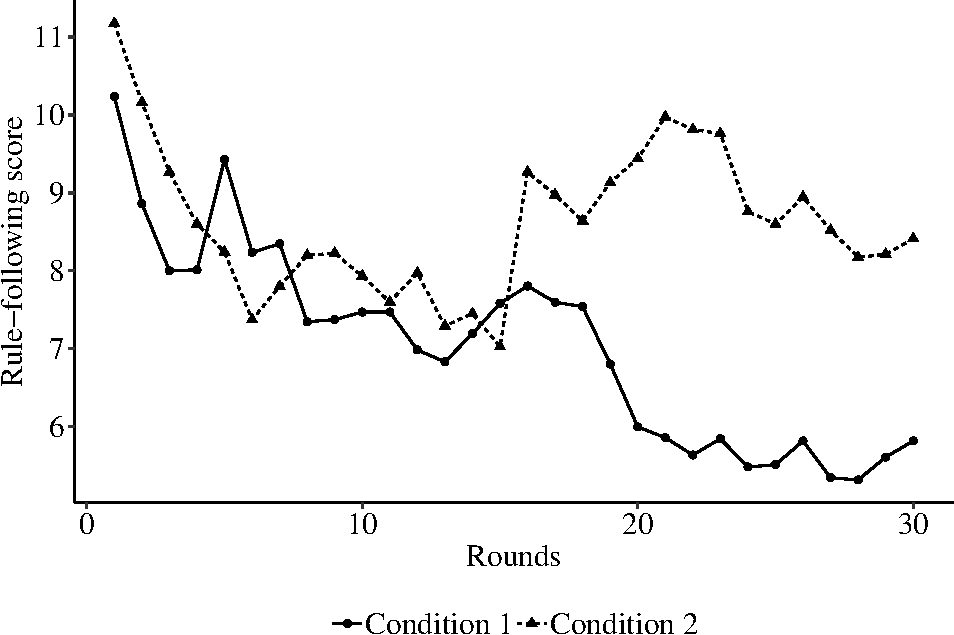
\includegraphics{Thesis_files/figure-latex/unnamed-chunk-1-1.pdf}
\emph{Figure 1.} Rule-following participants were chosen more in the
prosocial setting (dictator game) than in the corrupt setting (die-roll
game). In the first 15 rounds of condition one, participants played the
dictator game and in the remaining 15 rounds the die-roll game. In
condition two, this order was reversed.

\hypertarget{h2-transitioning-to-differing-settings}{%
\subsection{H2: Transitioning to Differing
Settings}\label{h2-transitioning-to-differing-settings}}

The order of social settings can introduce spill over effects and
therefore shape human behavior. For example, time trends of
rule-following behavior may spill over to another social setting and
anchor behavior. If rule following decreases due to a corrupt social
setting, for example, this decreased adherence may be carried over to a
prosocial setting in which following rules may be rewarded. However,
will we observe such anchoring effects?

Figure 1 reveals that there were no such expected anchoring effects and
that the trends of rule-following behavior when transitioning to another
setting are more complex than initially anticipated. Overall, rule
following decreased in the second half of the experiment more than in
the first half (\emph{b} = -1.83, 95\% CI{[}-2.18;-1.47{]}).
Interestingly, while rule following alone did not differ across the two
conditions (i.e., the order that the two settings follow; \emph{b} =
-1.83, 95\% CI{[}-2.18;-1.47{]}), conditions interacted with the order
of the settings where people were more rule following in the second half
of condition 2 (i.e., the dictator game) than in condition 1 (i.e., the
die-rolling game; \emph{b} = 2.51, 95\% CI{[}2.02;3.01{]}). This
interaction shows that even though there are no anchoring effects per
se, merely transitioning from one setting to the next, evokes
differential rule following behavior across settings in the direction we
predicted. However, this change may as well have been caused by
opportunism as people also had the chance to get selected as interaction
partners, inducing selection pressures.

{[}why?{]}

-discussion: why? - we expected - outcome: - in the corrupt setting,
steady decrease of rule following scores over time - in the prosocial
setting, steady increase of rule following scores over time - both
trends would be exacerbate when transitioning to them - because - - but
what happened

\begin{Shaded}
\begin{Highlighting}[]
\KeywordTok{setwd}\NormalTok{(}\StringTok{'/Users/sese/Desktop/Data/'}\NormalTok{)}
\NormalTok{result <-}\StringTok{ }\KeywordTok{read.table}\NormalTok{(}\StringTok{'result.csv'}\NormalTok{, }\DataTypeTok{header=}\NormalTok{T, }\DataTypeTok{sep=}\StringTok{','}\NormalTok{)}
\NormalTok{result <-}\StringTok{ }\NormalTok{result[,}\DecValTok{2}\OperatorTok{:}\KeywordTok{dim}\NormalTok{(result)[}\DecValTok{2}\NormalTok{]]}


\KeywordTok{library}\NormalTok{(ggplot2)}
\NormalTok{apatheme=}\KeywordTok{theme_bw}\NormalTok{()}\OperatorTok{+}
\StringTok{  }\KeywordTok{theme}\NormalTok{(}\DataTypeTok{panel.grid.major=}\KeywordTok{element_blank}\NormalTok{(),}
        \DataTypeTok{panel.grid.minor=}\KeywordTok{element_blank}\NormalTok{(),}
        \DataTypeTok{panel.border=}\KeywordTok{element_blank}\NormalTok{(),}
        \DataTypeTok{axis.line=}\KeywordTok{element_line}\NormalTok{(),}
        \DataTypeTok{text=}\KeywordTok{element_text}\NormalTok{(}\DataTypeTok{family=}\StringTok{'serif'}\NormalTok{, }\DataTypeTok{size =} \DecValTok{15}\NormalTok{),}
        \DataTypeTok{legend.text =} \KeywordTok{element_text}\NormalTok{(}\DataTypeTok{family =} \StringTok{'serif'}\NormalTok{, }\DataTypeTok{size =} \DecValTok{15}\NormalTok{),}
        \DataTypeTok{axis.text =} \KeywordTok{element_text}\NormalTok{(}\DataTypeTok{family =} \StringTok{'serif'}\NormalTok{, }\DataTypeTok{size =} \DecValTok{15}\NormalTok{, }\DataTypeTok{colour =} \StringTok{'black'}\NormalTok{),}
        \DataTypeTok{legend.title=}\KeywordTok{element_blank}\NormalTok{(),}
        \DataTypeTok{plot.caption =} \KeywordTok{element_text}\NormalTok{(}\DataTypeTok{hjust =} \FloatTok{0.05}\NormalTok{, }\DataTypeTok{family =} \StringTok{'serif'}\NormalTok{, }\DataTypeTok{size =} \DecValTok{15}\NormalTok{)) }

\NormalTok{data <-}\StringTok{ }\KeywordTok{expand.grid}\NormalTok{(}\DataTypeTok{type =} \DecValTok{1}\OperatorTok{:}\DecValTok{2}\NormalTok{, }\DataTypeTok{order =} \DecValTok{1}\OperatorTok{:}\DecValTok{2}\NormalTok{, }\DataTypeTok{rf =} \OtherTok{NA}\NormalTok{)}
\NormalTok{data}\OperatorTok{$}\NormalTok{rf[}\DecValTok{1}\NormalTok{] <-}\StringTok{ }\KeywordTok{mean}\NormalTok{(result}\OperatorTok{$}\NormalTok{rulefollowing[result}\OperatorTok{$}\NormalTok{order }\OperatorTok{==}\StringTok{ }\KeywordTok{levels}\NormalTok{(result}\OperatorTok{$}\NormalTok{order)[}\DecValTok{1}\NormalTok{] }\OperatorTok{&}\StringTok{ }\NormalTok{result}\OperatorTok{$}\NormalTok{type }\OperatorTok{==}\StringTok{ 'dictator'}\NormalTok{], }\DataTypeTok{na.rm =}\NormalTok{ T)}
\NormalTok{data}\OperatorTok{$}\NormalTok{rf[}\DecValTok{2}\NormalTok{] <-}\StringTok{ }\KeywordTok{mean}\NormalTok{(result}\OperatorTok{$}\NormalTok{rulefollowing[result}\OperatorTok{$}\NormalTok{order }\OperatorTok{==}\StringTok{ }\KeywordTok{levels}\NormalTok{(result}\OperatorTok{$}\NormalTok{order)[}\DecValTok{1}\NormalTok{] }\OperatorTok{&}\StringTok{ }\NormalTok{result}\OperatorTok{$}\NormalTok{type }\OperatorTok{==}\StringTok{ 'dieroll'}\NormalTok{], }\DataTypeTok{na.rm =}\NormalTok{ T)}
\NormalTok{data}\OperatorTok{$}\NormalTok{rf[}\DecValTok{3}\NormalTok{] <-}\StringTok{ }\KeywordTok{mean}\NormalTok{(result}\OperatorTok{$}\NormalTok{rulefollowing[result}\OperatorTok{$}\NormalTok{order }\OperatorTok{==}\StringTok{ }\KeywordTok{levels}\NormalTok{(result}\OperatorTok{$}\NormalTok{order)[}\DecValTok{2}\NormalTok{] }\OperatorTok{&}\StringTok{ }\NormalTok{result}\OperatorTok{$}\NormalTok{type }\OperatorTok{==}\StringTok{ 'dictator'}\NormalTok{], }\DataTypeTok{na.rm =}\NormalTok{ T)}
\NormalTok{data}\OperatorTok{$}\NormalTok{rf[}\DecValTok{4}\NormalTok{] <-}\StringTok{ }\KeywordTok{mean}\NormalTok{(result}\OperatorTok{$}\NormalTok{rulefollowing[result}\OperatorTok{$}\NormalTok{order }\OperatorTok{==}\StringTok{ }\KeywordTok{levels}\NormalTok{(result}\OperatorTok{$}\NormalTok{order)[}\DecValTok{2}\NormalTok{] }\OperatorTok{&}\StringTok{ }\NormalTok{result}\OperatorTok{$}\NormalTok{type }\OperatorTok{==}\StringTok{ 'dieroll'}\NormalTok{], }\DataTypeTok{na.rm =}\NormalTok{ T)}

\NormalTok{data}\OperatorTok{$}\NormalTok{type <-}\StringTok{ }\KeywordTok{ifelse}\NormalTok{(data}\OperatorTok{$}\NormalTok{type }\OperatorTok{==}\StringTok{ }\DecValTok{1}\NormalTok{, }\StringTok{'prosocial'}\NormalTok{, }\StringTok{'corrupt'}\NormalTok{)}
\NormalTok{data}\OperatorTok{$}\NormalTok{order <-}\StringTok{ }\KeywordTok{ifelse}\NormalTok{(data}\OperatorTok{$}\NormalTok{order }\OperatorTok{==}\StringTok{ }\DecValTok{1}\NormalTok{, }\StringTok{'first half'}\NormalTok{, }\StringTok{'second half'}\NormalTok{)}

\KeywordTok{library}\NormalTok{(ggplot2)}
\KeywordTok{ggplot}\NormalTok{(data, }\KeywordTok{aes}\NormalTok{(}\DataTypeTok{x =}\NormalTok{ order, }\DataTypeTok{y =}\NormalTok{ rf, }\DataTypeTok{fill =}\NormalTok{ type)) }\OperatorTok{+}
\StringTok{  }\KeywordTok{geom_bar}\NormalTok{(}\DataTypeTok{stat =} \StringTok{'identity'}\NormalTok{, }\DataTypeTok{position=}\KeywordTok{position_dodge}\NormalTok{(), }\DataTypeTok{color =} \StringTok{'black'}\NormalTok{) }\OperatorTok{+}
\StringTok{  }\KeywordTok{labs}\NormalTok{(}
    \CommentTok{# caption = "Figure 1. Rule-following participants were chosen more in the \textbackslash{}ndictator game (fair setting) than in the die-roll game (corrupt setting).",}
    \DataTypeTok{x =} \StringTok{""}\NormalTok{, }\DataTypeTok{y =} \StringTok{"rule-following score"}\NormalTok{) }\OperatorTok{+}
\StringTok{  }\KeywordTok{scale_fill_manual}\NormalTok{(}\DataTypeTok{values=}\KeywordTok{c}\NormalTok{(}\StringTok{'#222222'}\NormalTok{,}\StringTok{'#ffffff'}\NormalTok{)) }\OperatorTok{+}
\StringTok{  }\NormalTok{apatheme }\OperatorTok{+}
\StringTok{  }\KeywordTok{scale_y_continuous}\NormalTok{(}\DataTypeTok{expand =} \KeywordTok{c}\NormalTok{(}\DecValTok{0}\NormalTok{, }\DecValTok{0}\NormalTok{), }\DataTypeTok{limits =} \KeywordTok{c}\NormalTok{(}\DecValTok{0}\NormalTok{, }\DecValTok{11}\NormalTok{))}
\end{Highlighting}
\end{Shaded}

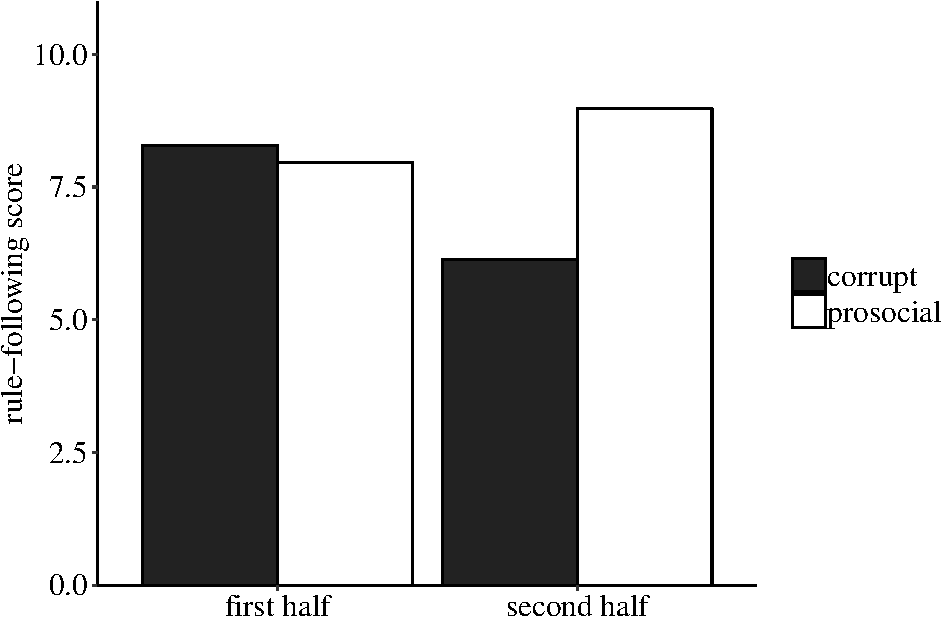
\includegraphics{Thesis_files/figure-latex/unnamed-chunk-2-1.pdf}
\emph{Figure 2.} In the first half, rule following was not different for
the corrupt and prosocial setting but was different in the second half.
While the corrupt setting promoted abandoning rules, the prosocial
setting facilitated following rules.

\hypertarget{h3-choosing-the-trustworthy}{%
\subsection{H3: Choosing the
Trustworthy}\label{h3-choosing-the-trustworthy}}

H3: main effects of selected\emph{type (full, half 1 and half 2) - full
- selected + (}b* = 1.25, 95\% CI{[}0.88;1.63{]}) - type + (\emph{b} =
-0.46, 95\% CI{[}-0.87;-0.05{]}) - interaction + (\emph{b} = -1.38, 95\%
CI{[}-1.92;-0.85{]}) - half 1 - selected + (\emph{b} = 1.45, 95\%
CI{[}0.92;1.97{]}) - type - (\emph{b} = 1.34, 95\% CI{[}-0.91;3.60{]}) -
interaction + (\emph{b} = -1.89, 95\% CI{[}-2.64;-1.13{]}) - half 2 -
selected + (\emph{b} = 1.35, 95\% CI{[}0.87;1.83{]}) - type - (\emph{b}
= -2.50, 95\% CI{[}-5.22;0.21{]}) - interaction - (\emph{b} = -0.60,
95\% CI{[}-1.30;0.10{]})

\begin{Shaded}
\begin{Highlighting}[]
\CommentTok{# h3}
\CommentTok{# rm(list = ls())}
\KeywordTok{setwd}\NormalTok{(}\StringTok{'/Users/sese/Desktop/Data/'}\NormalTok{)}
\NormalTok{result <-}\StringTok{ }\KeywordTok{read.table}\NormalTok{(}\StringTok{'result.csv'}\NormalTok{, }\DataTypeTok{header=}\NormalTok{T, }\DataTypeTok{sep=}\StringTok{','}\NormalTok{)}
\NormalTok{result <-}\StringTok{ }\NormalTok{result[,}\DecValTok{2}\OperatorTok{:}\KeywordTok{dim}\NormalTok{(result)[}\DecValTok{2}\NormalTok{]]}

\NormalTok{create_set <-}\StringTok{ }\ControlFlowTok{function}\NormalTok{(part) \{}
  
  \KeywordTok{library}\NormalTok{(plyr)}
  
\NormalTok{  result_half1 <-}\StringTok{ }\KeywordTok{subset}\NormalTok{(result, result}\OperatorTok{$}\NormalTok{round }\OperatorTok{<=}\StringTok{ }\DecValTok{15}\NormalTok{)}
\NormalTok{  result_half2 <-}\StringTok{ }\KeywordTok{subset}\NormalTok{(result, result}\OperatorTok{$}\NormalTok{round }\OperatorTok{>=}\StringTok{ }\DecValTok{16}\NormalTok{)}
\NormalTok{  set <-}\StringTok{ }\KeywordTok{c}\NormalTok{(}\StringTok{'result_half1'}\NormalTok{, }\StringTok{'result_half2'}\NormalTok{, }\StringTok{'result'}\NormalTok{)}
  
\NormalTok{  data}\OperatorTok{$}\NormalTok{rulefollowing[}\DecValTok{1}\NormalTok{] <-}\StringTok{ }\KeywordTok{mean}\NormalTok{(}\KeywordTok{eval}\NormalTok{(}\KeywordTok{parse}\NormalTok{(}\DataTypeTok{text =} \KeywordTok{paste}\NormalTok{(set[part])))}\OperatorTok{$}\NormalTok{rulefollowing[result}\OperatorTok{$}\NormalTok{type }\OperatorTok{==}\StringTok{ }\KeywordTok{levels}\NormalTok{(result}\OperatorTok{$}\NormalTok{type)[}\DecValTok{1}\NormalTok{] }\OperatorTok{&}\StringTok{ }\NormalTok{result}\OperatorTok{$}\NormalTok{selected }\OperatorTok{==}\StringTok{ }\KeywordTok{levels}\NormalTok{(result}\OperatorTok{$}\NormalTok{selected)[}\DecValTok{1}\NormalTok{]], }\DataTypeTok{na.rm =}\NormalTok{ T)}
\NormalTok{  data}\OperatorTok{$}\NormalTok{rulefollowing[}\DecValTok{2}\NormalTok{] <-}\StringTok{ }\KeywordTok{mean}\NormalTok{(}\KeywordTok{eval}\NormalTok{(}\KeywordTok{parse}\NormalTok{(}\DataTypeTok{text =} \KeywordTok{paste}\NormalTok{(set[part])))}\OperatorTok{$}\NormalTok{rulefollowing[result}\OperatorTok{$}\NormalTok{type }\OperatorTok{==}\StringTok{ }\KeywordTok{levels}\NormalTok{(result}\OperatorTok{$}\NormalTok{type)[}\DecValTok{2}\NormalTok{] }\OperatorTok{&}\StringTok{ }\NormalTok{result}\OperatorTok{$}\NormalTok{selected }\OperatorTok{==}\StringTok{ }\KeywordTok{levels}\NormalTok{(result}\OperatorTok{$}\NormalTok{selected)[}\DecValTok{1}\NormalTok{]], }\DataTypeTok{na.rm =}\NormalTok{ T)}
\NormalTok{  data}\OperatorTok{$}\NormalTok{rulefollowing[}\DecValTok{3}\NormalTok{] <-}\StringTok{ }\KeywordTok{mean}\NormalTok{(}\KeywordTok{eval}\NormalTok{(}\KeywordTok{parse}\NormalTok{(}\DataTypeTok{text =} \KeywordTok{paste}\NormalTok{(set[part])))}\OperatorTok{$}\NormalTok{rulefollowing[result}\OperatorTok{$}\NormalTok{type }\OperatorTok{==}\StringTok{ }\KeywordTok{levels}\NormalTok{(result}\OperatorTok{$}\NormalTok{type)[}\DecValTok{1}\NormalTok{] }\OperatorTok{&}\StringTok{ }\NormalTok{result}\OperatorTok{$}\NormalTok{selected }\OperatorTok{==}\StringTok{ }\KeywordTok{levels}\NormalTok{(result}\OperatorTok{$}\NormalTok{selected)[}\DecValTok{2}\NormalTok{]], }\DataTypeTok{na.rm =}\NormalTok{ T)}
\NormalTok{  data}\OperatorTok{$}\NormalTok{rulefollowing[}\DecValTok{4}\NormalTok{] <-}\StringTok{ }\KeywordTok{mean}\NormalTok{(}\KeywordTok{eval}\NormalTok{(}\KeywordTok{parse}\NormalTok{(}\DataTypeTok{text =} \KeywordTok{paste}\NormalTok{(set[part])))}\OperatorTok{$}\NormalTok{rulefollowing[result}\OperatorTok{$}\NormalTok{type }\OperatorTok{==}\StringTok{ }\KeywordTok{levels}\NormalTok{(result}\OperatorTok{$}\NormalTok{type)[}\DecValTok{2}\NormalTok{] }\OperatorTok{&}\StringTok{ }\NormalTok{result}\OperatorTok{$}\NormalTok{selected }\OperatorTok{==}\StringTok{ }\KeywordTok{levels}\NormalTok{(result}\OperatorTok{$}\NormalTok{selected)[}\DecValTok{2}\NormalTok{]], }\DataTypeTok{na.rm =}\NormalTok{ T)}
  
\NormalTok{  data}\OperatorTok{$}\NormalTok{type <-}\StringTok{ }\KeywordTok{ifelse}\NormalTok{(data}\OperatorTok{$}\NormalTok{type }\OperatorTok{==}\StringTok{ }\DecValTok{1}\NormalTok{, }\StringTok{'DG'}\NormalTok{, }\StringTok{'DDG'}\NormalTok{)}
\NormalTok{  data}\OperatorTok{$}\NormalTok{selected <-}\StringTok{ }\KeywordTok{ifelse}\NormalTok{(data}\OperatorTok{$}\NormalTok{selected }\OperatorTok{==}\StringTok{ }\DecValTok{0}\NormalTok{, }\StringTok{'Not selected'}\NormalTok{, }\StringTok{'Selected'}\NormalTok{)}
  
  \KeywordTok{return}\NormalTok{(data)}
\NormalTok{\}}


\ControlFlowTok{for}\NormalTok{(i }\ControlFlowTok{in} \DecValTok{1}\OperatorTok{:}\DecValTok{3}\NormalTok{) \{}
\NormalTok{  data <-}\StringTok{ }\KeywordTok{expand.grid}\NormalTok{(}\DataTypeTok{type =} \DecValTok{1}\OperatorTok{:}\DecValTok{2}\NormalTok{, }\DataTypeTok{selected =} \DecValTok{0}\OperatorTok{:}\DecValTok{1}\NormalTok{, }\DataTypeTok{rulefollowing =} \OtherTok{NA}\NormalTok{)}
\NormalTok{  data <-}\StringTok{ }\KeywordTok{create_set}\NormalTok{(i)}
  \KeywordTok{print}\NormalTok{(i)}
  \KeywordTok{print}\NormalTok{(data)}
  
  \ControlFlowTok{if}\NormalTok{(i }\OperatorTok{==}\StringTok{ }\DecValTok{1}\NormalTok{) \{}
    \KeywordTok{library}\NormalTok{(ggplot2)}
\NormalTok{    plot1 <-}\StringTok{ }\KeywordTok{ggplot}\NormalTok{(data, }\KeywordTok{aes}\NormalTok{(}\DataTypeTok{x =}\NormalTok{ type, }\DataTypeTok{y =}\NormalTok{ rulefollowing, }\DataTypeTok{fill =}\NormalTok{ selected)) }\OperatorTok{+}
\StringTok{      }\KeywordTok{geom_bar}\NormalTok{(}\DataTypeTok{stat =} \StringTok{'identity'}\NormalTok{, }\DataTypeTok{position=}\KeywordTok{position_dodge}\NormalTok{(), }\DataTypeTok{color =} \StringTok{'black'}\NormalTok{) }\OperatorTok{+}
\StringTok{      }\KeywordTok{labs}\NormalTok{(}
        \CommentTok{# caption = "Figure 1. Rule-following participants were chosen more in the \textbackslash{}ndictator game (fair setting) than in the die-roll game (corrupt setting).",}
        \DataTypeTok{x =} \StringTok{""}\NormalTok{, }\DataTypeTok{y =} \StringTok{"rule-following score"}\NormalTok{) }\OperatorTok{+}
\StringTok{      }\KeywordTok{scale_fill_manual}\NormalTok{(}\DataTypeTok{values=}\KeywordTok{c}\NormalTok{(}\StringTok{'#222222'}\NormalTok{,}\StringTok{'#ffffff'}\NormalTok{)) }\OperatorTok{+}\StringTok{ }
\StringTok{      }\NormalTok{apatheme }\OperatorTok{+}
\StringTok{      }\KeywordTok{scale_y_continuous}\NormalTok{(}\DataTypeTok{expand =} \KeywordTok{c}\NormalTok{(}\DecValTok{0}\NormalTok{, }\DecValTok{0}\NormalTok{), }\DataTypeTok{limits =} \KeywordTok{c}\NormalTok{(}\DecValTok{0}\NormalTok{, }\DecValTok{11}\NormalTok{))}
\NormalTok{  \}}
  
  \ControlFlowTok{if}\NormalTok{(i }\OperatorTok{==}\StringTok{ }\DecValTok{2}\NormalTok{) \{}
    \KeywordTok{library}\NormalTok{(ggplot2)}
\NormalTok{    plot2 <-}\StringTok{ }\KeywordTok{ggplot}\NormalTok{(data, }\KeywordTok{aes}\NormalTok{(}\DataTypeTok{x =}\NormalTok{ type, }\DataTypeTok{y =}\NormalTok{ rulefollowing, }\DataTypeTok{fill =}\NormalTok{ selected)) }\OperatorTok{+}
\StringTok{      }\KeywordTok{geom_bar}\NormalTok{(}\DataTypeTok{stat =} \StringTok{'identity'}\NormalTok{, }\DataTypeTok{position=}\KeywordTok{position_dodge}\NormalTok{(), }\DataTypeTok{color =} \StringTok{'black'}\NormalTok{) }\OperatorTok{+}
\StringTok{      }\KeywordTok{labs}\NormalTok{(}
        \CommentTok{# caption = "Figure 1. Rule-following participants were chosen more in the \textbackslash{}ndictator game (fair setting) than in the die-roll game (corrupt setting).",}
        \DataTypeTok{x =} \StringTok{""}\NormalTok{, }\DataTypeTok{y =} \StringTok{"rule-following score"}\NormalTok{) }\OperatorTok{+}
\StringTok{      }\KeywordTok{scale_fill_manual}\NormalTok{(}\DataTypeTok{values=}\KeywordTok{c}\NormalTok{(}\StringTok{'#222222'}\NormalTok{,}\StringTok{'#ffffff'}\NormalTok{)) }\OperatorTok{+}\StringTok{ }
\StringTok{      }\NormalTok{apatheme }\OperatorTok{+}
\StringTok{      }\KeywordTok{scale_y_continuous}\NormalTok{(}\DataTypeTok{expand =} \KeywordTok{c}\NormalTok{(}\DecValTok{0}\NormalTok{, }\DecValTok{0}\NormalTok{), }\DataTypeTok{limits =} \KeywordTok{c}\NormalTok{(}\DecValTok{0}\NormalTok{, }\DecValTok{11}\NormalTok{))}
\NormalTok{  \} }
  
  \ControlFlowTok{if}\NormalTok{(i }\OperatorTok{==}\StringTok{ }\DecValTok{3}\NormalTok{) \{}
    \KeywordTok{library}\NormalTok{(ggplot2)}
\NormalTok{    plot3 <-}\StringTok{ }\KeywordTok{ggplot}\NormalTok{(data, }\KeywordTok{aes}\NormalTok{(}\DataTypeTok{x =}\NormalTok{ type, }\DataTypeTok{y =}\NormalTok{ rulefollowing, }\DataTypeTok{fill =}\NormalTok{ selected)) }\OperatorTok{+}
\StringTok{      }\KeywordTok{geom_bar}\NormalTok{(}\DataTypeTok{stat =} \StringTok{'identity'}\NormalTok{, }\DataTypeTok{position=}\KeywordTok{position_dodge}\NormalTok{(), }\DataTypeTok{color =} \StringTok{'black'}\NormalTok{) }\OperatorTok{+}
\StringTok{      }\KeywordTok{labs}\NormalTok{(}
        \CommentTok{# caption = "Figure 1. Rule-following participants were chosen more in the \textbackslash{}ndictator game (fair setting) than in the die-roll game (corrupt setting).",}
        \DataTypeTok{x =} \StringTok{""}\NormalTok{, }\DataTypeTok{y =} \StringTok{"rule-following score"}\NormalTok{) }\OperatorTok{+}
\StringTok{      }\KeywordTok{scale_fill_manual}\NormalTok{(}\DataTypeTok{values=}\KeywordTok{c}\NormalTok{(}\StringTok{'#222222'}\NormalTok{,}\StringTok{'#ffffff'}\NormalTok{)) }\OperatorTok{+}\StringTok{ }
\StringTok{      }\NormalTok{apatheme }\OperatorTok{+}
\StringTok{      }\KeywordTok{scale_y_continuous}\NormalTok{(}\DataTypeTok{expand =} \KeywordTok{c}\NormalTok{(}\DecValTok{0}\NormalTok{, }\DecValTok{0}\NormalTok{), }\DataTypeTok{limits =} \KeywordTok{c}\NormalTok{(}\DecValTok{0}\NormalTok{, }\DecValTok{11}\NormalTok{))}
\NormalTok{  \}}
\NormalTok{\}}
\end{Highlighting}
\end{Shaded}

\begin{verbatim}
## [1] 1
##   type     selected rulefollowing
## 1   DG Not selected      6.972171
## 2  DDG Not selected      8.371429
## 3   DG     Selected      8.942699
## 4  DDG     Selected      8.244595
## [1] 2
##   type     selected rulefollowing
## 1   DG Not selected      5.820037
## 2  DDG Not selected      8.831169
## 3   DG     Selected      6.447320
## 4  DDG     Selected      9.050000
## [1] 3
##   type     selected rulefollowing
## 1   DG Not selected      7.286157
## 2  DDG Not selected      7.582329
## 3   DG     Selected      9.409863
## 4  DDG     Selected      7.054184
\end{verbatim}

\begin{Shaded}
\begin{Highlighting}[]
\KeywordTok{require}\NormalTok{(gridExtra)}
\end{Highlighting}
\end{Shaded}

\begin{verbatim}
## Loading required package: gridExtra
\end{verbatim}

\begin{Shaded}
\begin{Highlighting}[]
\KeywordTok{grid.arrange}\NormalTok{(plot1, plot2, plot3, }\DataTypeTok{nrow =} \DecValTok{3}\NormalTok{)}
\end{Highlighting}
\end{Shaded}

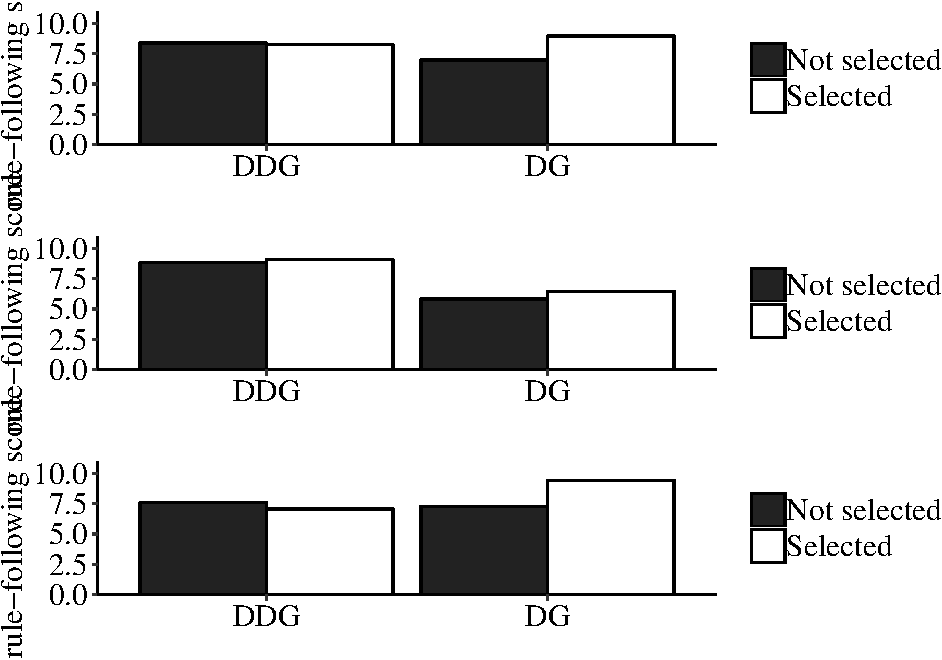
\includegraphics{Thesis_files/figure-latex/unnamed-chunk-3-1.pdf}
\emph{Figure 3.} {[}add description{]}

\hypertarget{dump-section}{%
\section{Dump Section}\label{dump-section}}

\hypertarget{results-1}{%
\subsection{Results}\label{results-1}}

H1: interaction between type\emph{round (full, half 1 and half 2) - full
- type - (}b* = -0.20, 95\% CI{[}-1.11;0.70{]}) - round + (\emph{b} =
-0.03, 95\% CI{[}-0.06;-0.00{]}) - interaction + (\emph{b} = -0.07, 95\%
CI{[}-0.12;-0.01{]}) - half 1 - type - (\emph{b} = -0.65, 95\%
CI{[}-1.65;2.94{]}) - round + (\emph{b} = -0.17, 95\%
CI{[}-0.22;-0.11{]}) - interaction - (\emph{b} = -0.04, 95\%
CI{[}-0.12;-0.04{]}) - half 2 - type - (\emph{b} = -0.91, 95\%
CI{[}-4.00;2.18{]}) - round + (\emph{b} = -0.07, 95\%
CI{[}-0.12;-0.03{]}) - interaction + (\emph{b} = -0.08, 95\%
CI{[}-0.15;-0.02{]}) H2: interaction between type\emph{order (full, +/-
interaction) - full - interaction - type + (}b* = -1.26, 95\%
CI{[}-1.50;-1.01{]}) - order + (\emph{b} = -0.57, 95\%
CI{[}-0.82;-0.32{]}) - full + interaction - type- (\emph{b} = 0.33, 95\%
CI{[}-1.97;2.63{]}) - order - (\emph{b} = 1.02, 95\% CI{[}-1.28;3.31{]})
- interaction - (\emph{b} = -3.17, 95\% CI{[}-7.74;1.40{]}) - full 4
condition\emph{order (full) - condition - (}b* = 0.33, 95\%
CI{[}-1.97;2.63{]}) - order + (\emph{b} = -1.83, 95\%
CI{[}-2.18;-1.47{]}) - interaction + (\emph{b} = 2.51, 95\%
CI{[}2.02;3.01{]})

\hypertarget{h1}{%
\subsection{H1}\label{h1}}

In line with our expectation, norms of rule following were established
in both settings as shown in Figure 1. However, to our surprise,
rule-following scores overall decreased over time regardless the setting
(\emph{b} = -0.16, 95\% CI{[}-0.22;-0.11{]}) showing that the expected
diverging pressures we predicted did not arise. So, while rule following
consistently decreased in the corrupt setting as we expected,
{[}stats{]}, with an average minimum rule-following score = 5.32 in
round 28, rule following also decreased in the prosocial setting with
rule following peaking at an average score = 9.97 in round 21. There was
no main effect for the settings variable in the first half, {[}stats{]},
and we did not find an interaction effect between both settings and
rounds either, {[}stats{]}. However, in the second half differences
emerged and the order of the two settings (i.e., transitioning from one
setting to another) may have influenced rule following behavior in both
settings.

However, merely transitioning from one setting to another seemed
temporarily increase rule following in the corrupt setting even if not
remarkably, {[}stats{]}. When transitioning to the prosocial setting,
there was a strong increase in rule-following scores, {[}stats{]},
followed by the decreasing trend mentioned above.

In our experiment, we measured rule-following behavior as an interval
variable ranging from 0 to 15, which translates to the number of a
participant following the rule.

\hypertarget{h2-transitioning-to-differing-settings-1}{%
\subsection{H2: Transitioning to Differing
Settings}\label{h2-transitioning-to-differing-settings-1}}

Interestingly, in the first 15 rounds of the experiment, rule-following
scores do not differ across the two settings over time, \emph{b} =
-0.04, 95\% CI{[}-0.12;0.04{]}. Over the remaining 15 rounds, however,
the scores did differ, \emph{b} = -0.08, 95\% CI{[}-0.15;-0.02{]}.
Therefore, it seems that merely transitioning from one setting to the
next caused rule-following scores to differ, possibly, because the
transition made the incentive structures more salient.

Overall, participants followed rules less in both the corrupt setting
(\emph{b} = -1.26, 95\% CI{[}-1.50;-1.01{]}) and the second half of the
experiment (\emph{b} = -0.57, 95\% CI{[}-0.82;-0.32{]}). However, when
including the interaction term, none of the effects predicted rule
following behavior; not the variable setting (\emph{b} = 0.33, 95\%
CI{[}-1.97;2.63{]}), order (\emph{b} = 1.02, 95\% CI{[}-1.28;3.31{]}),
or the interaction term (\emph{b} = -3.17, 95\% CI{[}-7.74;1.40{]}).

Over the first 15 rounds of our experiment, the trends of the scores did
not differ across the two settings ( \emph{b} = -0.04, 95\%
CI{[}-0.12;0.04{]}) but did differ over the 15 rounds after (\emph{b} =
-0.08, 95\% CI{[}-0.15;-0.02{]}). Specifically, in the corrupt setting,
rule following decreased even further in the second half as predicted,
{[}stats{]}. However, in the prosocial setting, rule-following scores
deviated from our expectations. First of all, scores did not increase
but decrease in the first half, {[}stats{]}. Then, when transitioning to
the prosocial setting, scores rapidly increased, {[}stats{]}, and
consistently decreased thereafter as part of the overall decreasing
trend, {[}stats{]}.

\hypertarget{h3-choosing-the-trustworthy-1}{%
\subsection{H3: Choosing the
Trustworthy}\label{h3-choosing-the-trustworthy-1}}

\hypertarget{general-discussion}{%
\subsection{General Discussion}\label{general-discussion}}

Given all these results, why do we observe an overall decreasing trend?

\hypertarget{establishing-norms-of-rule-following}{%
\section{Establishing norms of rule
following}\label{establishing-norms-of-rule-following}}

Social settings

\begin{itemize}
\tightlist
\item
  we predict

  \begin{itemize}
  \item
    rule-following increases in the prosocial setting and decreases in
    the corrupt setting
  \item
  \end{itemize}
\item
  Figure 1 shows the trends of rule-following scores over time.
\end{itemize}

\hypertarget{social-environments-anchor-rule-following-behavior}{%
\section{Social environments anchor rule following
behavior}\label{social-environments-anchor-rule-following-behavior}}

\hypertarget{choosing-partners-shapes-rule-following-behavior}{%
\section{Choosing partners shapes rule following
behavior}\label{choosing-partners-shapes-rule-following-behavior}}

In line with our expectations, people became less rule following over
time in the corrupt setting (H1a), {[}stats{]}. Surprisingly,

H1 - H1a: confirmed - H1b: not confirmed - surprisingly, high onset of
rule-following scores - also, surprisingly, overall downward trend of
rule-following behavior H2 - H2a:

\begin{Shaded}
\begin{Highlighting}[]
\KeywordTok{setwd}\NormalTok{(}\StringTok{'/Users/sese/Desktop/Data'}\NormalTok{)}
\NormalTok{result <-}\StringTok{ }\KeywordTok{read.table}\NormalTok{(}\StringTok{'result.csv'}\NormalTok{, }\DataTypeTok{header =}\NormalTok{ T, }\DataTypeTok{sep =} \StringTok{','}\NormalTok{)}
\NormalTok{result <-}\StringTok{ }\NormalTok{result[,}\DecValTok{2}\OperatorTok{:}\KeywordTok{dim}\NormalTok{(result)[}\DecValTok{2}\NormalTok{]]}

\CommentTok{# Model}
\KeywordTok{library}\NormalTok{(lme4)}
\end{Highlighting}
\end{Shaded}

\begin{verbatim}
## Warning: package 'lme4' was built under R version 3.5.2
\end{verbatim}

\begin{verbatim}
## Loading required package: Matrix
\end{verbatim}

\begin{Shaded}
\begin{Highlighting}[]
\NormalTok{model <-}\StringTok{ }\KeywordTok{lmer}\NormalTok{(rulefollowing }\OperatorTok{~}\StringTok{ }\DecValTok{1} \OperatorTok{+}\StringTok{ }\NormalTok{type}\OperatorTok{*}\NormalTok{round}\OperatorTok{*}\NormalTok{order }\OperatorTok{+}\StringTok{ }\NormalTok{type}\OperatorTok{*}\NormalTok{selected }\OperatorTok{+}\StringTok{ }\NormalTok{(}\DecValTok{1} \OperatorTok{|}\StringTok{ }\NormalTok{group}\OperatorTok{/}\NormalTok{subject),}
              \DataTypeTok{REML =}\NormalTok{ T,}
              \DataTypeTok{data =}\NormalTok{ result)}
\end{Highlighting}
\end{Shaded}

\begin{verbatim}
## Warning in checkConv(attr(opt, "derivs"), opt$par, ctrl =
## control$checkConv, : Model failed to converge with max|grad| = 0.00979702
## (tol = 0.002, component 1)
\end{verbatim}

\begin{Shaded}
\begin{Highlighting}[]
\KeywordTok{library}\NormalTok{(dplyr)}
\end{Highlighting}
\end{Shaded}

\begin{verbatim}
## Warning: package 'dplyr' was built under R version 3.5.2
\end{verbatim}

\begin{verbatim}
## 
## Attaching package: 'dplyr'
\end{verbatim}

\begin{verbatim}
## The following object is masked from 'package:gridExtra':
## 
##     combine
\end{verbatim}

\begin{verbatim}
## The following objects are masked from 'package:plyr':
## 
##     arrange, count, desc, failwith, id, mutate, rename, summarise,
##     summarize
\end{verbatim}

\begin{verbatim}
## The following objects are masked from 'package:stats':
## 
##     filter, lag
\end{verbatim}

\begin{verbatim}
## The following objects are masked from 'package:base':
## 
##     intersect, setdiff, setequal, union
\end{verbatim}

\begin{Shaded}
\begin{Highlighting}[]
\KeywordTok{library}\NormalTok{(knitr)}
\end{Highlighting}
\end{Shaded}

\begin{verbatim}
## Warning: package 'knitr' was built under R version 3.5.2
\end{verbatim}

\begin{Shaded}
\begin{Highlighting}[]
\KeywordTok{library}\NormalTok{(DT)}
\end{Highlighting}
\end{Shaded}

\begin{verbatim}
## Warning: package 'DT' was built under R version 3.5.2
\end{verbatim}

\begin{Shaded}
\begin{Highlighting}[]
\KeywordTok{library}\NormalTok{(xtable)}
\KeywordTok{kable}\NormalTok{(}\KeywordTok{summary}\NormalTok{(model)}\OperatorTok{$}\NormalTok{coefficients, }\DataTypeTok{caption =} \StringTok{'Random Intercepts Regression Results'}\NormalTok{)}
\end{Highlighting}
\end{Shaded}

\begin{longtable}[]{@{}lrrr@{}}
\caption{Random Intercepts Regression Results}\tabularnewline
\toprule
& Estimate & Std. Error & t value\tabularnewline
\midrule
\endfirsthead
\toprule
& Estimate & Std. Error & t value\tabularnewline
\midrule
\endhead
(Intercept) & 8.6147539 & 0.8714305 & 9.8857614\tabularnewline
typedieroll & 1.3292224 & 1.2205251 & 1.0890578\tabularnewline
round & -0.1624833 & 0.0290433 & -5.5945144\tabularnewline
ordersecond half & 0.9354480 & 1.3598086 & 0.6879262\tabularnewline
selectedselected & 1.2863618 & 0.1882421 & 6.8335513\tabularnewline
typedieroll:round & -0.0447477 & 0.0407526 & -1.0980309\tabularnewline
typedieroll:ordersecond half & -1.1203772 & 2.5249255 &
-0.4437268\tabularnewline
round:ordersecond half & 0.1028781 & 0.0406692 &
2.5296348\tabularnewline
typedieroll:selectedselected & -1.2835164 & 0.2687629 &
-4.7756463\tabularnewline
typedieroll:round:ordersecond half & -0.0533288 & 0.0575910 &
-0.9259920\tabularnewline
\bottomrule
\end{longtable}

\begin{Shaded}
\begin{Highlighting}[]
\KeywordTok{kable}\NormalTok{(}\KeywordTok{confint}\NormalTok{(model), }\DataTypeTok{caption =} \StringTok{'95% CIs of Regression'}\NormalTok{)}
\end{Highlighting}
\end{Shaded}

\begin{verbatim}
## Computing profile confidence intervals ...
\end{verbatim}

\begin{longtable}[]{@{}lrr@{}}
\caption{95\% CIs of Regression}\tabularnewline
\toprule
& 2.5 \% & 97.5 \%\tabularnewline
\midrule
\endfirsthead
\toprule
& 2.5 \% & 97.5 \%\tabularnewline
\midrule
\endhead
.sig01 & 2.2123608 & 3.0013274\tabularnewline
.sig02 & 2.9139770 & 4.6750756\tabularnewline
.sigma & 4.0326526 & 4.2075468\tabularnewline
(Intercept) & 6.9105110 & 10.3192501\tabularnewline
typedieroll & -1.0580569 & 3.7161854\tabularnewline
round & -0.2193653 & -0.1055995\tabularnewline
ordersecond half & -1.7179722 & 3.5889692\tabularnewline
selectedselected & 0.9178764 & 1.6553247\tabularnewline
typedieroll:round & -0.1245655 & 0.0350672\tabularnewline
typedieroll:ordersecond half & -6.0542938 & 3.8133791\tabularnewline
round:ordersecond half & 0.0232271 & 0.1825325\tabularnewline
typedieroll:selectedselected & -1.8103473 & -0.7570791\tabularnewline
typedieroll:round:ordersecond half & -0.1661252 &
0.0594655\tabularnewline
\emph{Note}. {[}add specifics{]} & &\tabularnewline
\bottomrule
\end{longtable}

\hypertarget{norms-of-when-to-follow-rules-and-when-not}{%
\subsection{Norms of when to follow rules and when
not}\label{norms-of-when-to-follow-rules-and-when-not}}

Figure 1 shows the trends of rule-following scores over time.
Surprisingly, participants became consistently less rule following over
time, {[}stats{]} but as expected, rule-following scores decreased more
in the corrupt setting than in the prosocial setting (H1), {[}stats{]}.

\begin{itemize}
\tightlist
\item
  dv scale and analysis
\item
  results
\end{itemize}

Figure 1 shows the trends of rule-following scores over time. Overall,
participants became consistently less rule following over time, \emph{b}
= -0.15, 95\% CI = {[}-0.18,-0.12{]} and as expected, rule-following
scores decreased in the corrupt setting (H1a), \emph{b} = 0.33, 95\% CI
= {[}-0.22,-0.88{]}. However, different from our expectations, in the
prosocial setting, rule following did not increase per se. Instead, past
round 15 where the setting changed, the baseline of rule-following
scores increased in the prosocial setting followed by the downward trend
of scores, \emph{b} = 3.20, 95\% CI = {[}0.87,5.53{]}. In the corrupt
setting, the change increases rule-following scores momentarily but not
remarkably. We can therefore observe change effects for both settings
but not like we expected.

\begin{itemize}
\tightlist
\item
  figures

  \begin{itemize}
  \tightlist
  \item
    number of sixes reported: selector vs decider
  \item
    selector vs decider, measures of corruption vs svo
  \end{itemize}
\end{itemize}

\hypertarget{discussion}{%
\section{Discussion}\label{discussion}}

\begin{itemize}
\tightlist
\item
  terms `selector' and `decider' confusing
\end{itemize}

\newpage

\hypertarget{references}{%
\section{References}\label{references}}

\begin{Shaded}
\begin{Highlighting}[]
\KeywordTok{r_refs}\NormalTok{(}\DataTypeTok{file =} \StringTok{"r-references.bib"}\NormalTok{)}
\end{Highlighting}
\end{Shaded}

\begingroup
\setlength{\parindent}{-0.5in}
\setlength{\leftskip}{0.5in}

\hypertarget{refs}{}
\leavevmode\hypertarget{ref-abele2014communal}{}%
Abele, Andrea E, and Bogdan Wojciszke. 2014. ``Communal and Agentic
Content in Social Cognition: A Dual Perspective Model.'' In
\emph{Advances in Experimental Social Psychology}, 50:195--255.
Elsevier.

\leavevmode\hypertarget{ref-abeler2014representative}{}%
Abeler, Johannes, Anke Becker, and Armin Falk. 2014. ``Representative
Evidence on Lying Costs.'' \emph{Journal of Public Economics} 113:
96--104.

\leavevmode\hypertarget{ref-abeler2019preferences}{}%
Abeler, Johannes, Daniele Nosenzo, and Collin Raymond. 2019.
``Preferences for Truth-Telling.'' \emph{Econometrica} 87 (4): 1115--53.

\leavevmode\hypertarget{ref-ades1996causes}{}%
Ades, Alberto, and Rafael Di Tella. 1996. ``The Causes and Consequences
of Corruption: A Review of Recent Empirical Contributions.'' \emph{IDs
Bulletin} 27 (2): 6--11.

\leavevmode\hypertarget{ref-andre2011evolution}{}%
André, Jean-Baptiste, and Nicolas Baumard. 2011. ``The Evolution of
Fairness in a Biological Market.'' \emph{Evolution: International
Journal of Organic Evolution} 65 (5): 1447--56.

\leavevmode\hypertarget{ref-R-gridExtra}{}%
Auguie, Baptiste. 2017. \emph{GridExtra: Miscellaneous Functions for
"Grid" Graphics}. \url{https://CRAN.R-project.org/package=gridExtra}.

\leavevmode\hypertarget{ref-R-papaja}{}%
Aust, Frederik, and Marius Barth. 2018. \emph{papaja: Create APA
Manuscripts with R Markdown}. \url{https://github.com/crsh/papaja}.

\leavevmode\hypertarget{ref-bahmani2005impact}{}%
Bahmani-Oskooee, Mohsen, and Gour G Goswami. 2005. ``The Impact of
Corruption on the Black Market Premium.'' \emph{Southern Economic
Journal}, 483--93.

\leavevmode\hypertarget{ref-barclay2013strategies}{}%
Barclay, Pat. 2013. ``Strategies for Cooperation in Biological Markets,
Especially for Humans.'' \emph{Evolution and Human Behavior} 34 (3):
164--75.

\leavevmode\hypertarget{ref-barclay2006partner}{}%
Barclay, Pat, and Robb Willer. 2006. ``Partner Choice Creates
Competitive Altruism in Humans.'' \emph{Proceedings of the Royal Society
B: Biological Sciences} 274 (1610): 749--53.

\leavevmode\hypertarget{ref-R-Matrix}{}%
Bates, Douglas, and Martin Maechler. 2018. \emph{Matrix: Sparse and
Dense Matrix Classes and Methods}.
\url{https://CRAN.R-project.org/package=Matrix}.

\leavevmode\hypertarget{ref-R-lme4}{}%
Bates, Douglas, Martin Mächler, Ben Bolker, and Steve Walker. 2015.
``Fitting Linear Mixed-Effects Models Using lme4.'' \emph{Journal of
Statistical Software} 67 (1): 1--48.
\url{https://doi.org/10.18637/jss.v067.i01}.

\leavevmode\hypertarget{ref-baumard2014tool}{}%
Baumard, Josselin, François Osiurak, Mathieu Lesourd, and Didier Le
Gall. 2014. ``Tool Use Disorders After Left Brain Damage.''
\emph{Frontiers in Psychology} 5: 473.

\leavevmode\hypertarget{ref-baumard2013mutualistic}{}%
Baumard, Nicolas, Jean-Baptiste André, and Dan Sperber. 2013. ``A
Mutualistic Approach to Morality: The Evolution of Fairness by Partner
Choice.'' \emph{Behavioral and Brain Sciences} 36 (1): 59--78.

\leavevmode\hypertarget{ref-chen2016otree}{}%
Chen, Daniel L, Martin Schonger, and Chris Wickens. 2016. ``OTree---an
Open-Source Platform for Laboratory, Online, and Field Experiments.''
\emph{Journal of Behavioral and Experimental Finance} 9: 88--97.

\leavevmode\hypertarget{ref-cialdini2001harnessing}{}%
Cialdini, Robert B. 2001. ``Harnessing the Science of Persuasion.''
\emph{Harvard Business Review} 79 (9): 72--81.

\leavevmode\hypertarget{ref-cottrell2007people}{}%
Cottrell, Catherine A, Steven L Neuberg, and Norman P Li. 2007. ``What
Do People Desire in Others? A Sociofunctional Perspective on the
Importance of Different Valued Characteristics.'' \emph{Journal of
Personality and Social Psychology} 92 (2): 208.

\leavevmode\hypertarget{ref-cukierman1989seigniorage}{}%
Cukierman, Alex, Sebastian Edwards, and Guido Tabellini. 1989.
``Seigniorage and Political Instability.'' National Bureau of Economic
Research.

\leavevmode\hypertarget{ref-R-xtable}{}%
Dahl, David B., David Scott, Charles Roosen, Arni Magnusson, and
Jonathan Swinton. 2018. \emph{Xtable: Export Tables to Latex or Html}.
\url{https://CRAN.R-project.org/package=xtable}.

\leavevmode\hypertarget{ref-efferson2016sustained}{}%
Efferson, Charles, Carlos P Roca, Sonja Vogt, and Dirk Helbing. 2016.
``Sustained Cooperation by Running Away from Bad Behavior.''
\emph{Evolution and Human Behavior} 37 (1): 1--9.

\leavevmode\hypertarget{ref-everett2016inference}{}%
Everett, Jim AC, David A Pizarro, and MJ Crockett. 2016. ``Inference of
Trustworthiness from Intuitive Moral Judgments.'' \emph{Journal of
Experimental Psychology: General} 145 (6): 772.

\leavevmode\hypertarget{ref-farwell2014media}{}%
Farwell, James P. 2014. ``The Media Strategy of Isis.'' \emph{Survival}
56 (6): 49--55.

\leavevmode\hypertarget{ref-fehr2003nature}{}%
Fehr, Ernst, and Urs Fischbacher. 2003. ``The Nature of Human
Altruism.'' \emph{Nature} 425 (6960): 785.

\leavevmode\hypertarget{ref-fehr2002altruistic}{}%
Fehr, Ernst, and Simon Gächter. 2002. ``Altruistic Punishment in
Humans.'' \emph{Nature} 415 (6868): 137.

\leavevmode\hypertarget{ref-fehr2004human}{}%
Fehr, Ernst, and Bettina Rockenbach. 2004. ``Human Altruism: Economic,
Neural, and Evolutionary Perspectives.'' \emph{Current Opinion in
Neurobiology} 14 (6): 784--90.

\leavevmode\hypertarget{ref-fischbacher2013lies}{}%
Fischbacher, Urs, and Franziska Föllmi-Heusi. 2013. ``Lies in
Disguise---an Experimental Study on Cheating.'' \emph{Journal of the
European Economic Association} 11 (3): 525--47.

\leavevmode\hypertarget{ref-freud1977introductory}{}%
Freud, Sigmund. 1977. \emph{Introductory Lectures on Psychoanalysis}. WW
Norton \& Company.

\leavevmode\hypertarget{ref-gausel2011concern}{}%
Gausel, Nicolay, and Colin Wayne Leach. 2011. ``Concern for Self-Image
and Social Image in the Management of Moral Failure: Rethinking Shame.''
\emph{European Journal of Social Psychology} 41 (4): 468--78.

\leavevmode\hypertarget{ref-gelman2006data}{}%
Gelman, Andrew, and Jennifer Hill. 2006. \emph{Data Analysis Using
Regression and Multilevel/Hierarchical Models}. Cambridge university
press.

\leavevmode\hypertarget{ref-gintis2003solving}{}%
Gintis, Herbert. 2003. ``Solving the Puzzle of Prosociality.''
\emph{Rationality and Society} 15 (2): 155--87.

\leavevmode\hypertarget{ref-goodman2015volkswagen}{}%
Goodman, Leah M. 2015. ``Why Volkswagen Cheated.'' \emph{Newsweek
Global} 165 (23): 14.

\leavevmode\hypertarget{ref-goodwin2015moral}{}%
Goodwin, Geoffrey P. 2015. ``Moral Character in Person Perception.''
\emph{Current Directions in Psychological Science} 24 (1): 38--44.

\leavevmode\hypertarget{ref-dsanjeev1998does}{}%
Gupta, Jenny dSanjeev, Hamid Davoodi, and Rosa Alonso-Terme. 1998.
\emph{Does Corruption Affect Income Inequality and Poverty?}
International Monetary Fund.

\leavevmode\hypertarget{ref-gurven2000s}{}%
Gurven, Michael, Wesley Allen-Arave, Kim Hill, and Magdalena Hurtado.
2000. ```It's a Wonderful Life': Signaling Generosity Among the Ache of
Paraguay.'' \emph{Evolution and Human Behavior} 21 (4): 263--82.

\leavevmode\hypertarget{ref-hirschman1987people}{}%
Hirschman, Elizabeth C. 1987. ``People as Products: Analysis of a
Complex Marketing Exchange.'' \emph{Journal of Marketing} 51 (1):
98--108.

\leavevmode\hypertarget{ref-hoffman1977moral}{}%
Hoffman, Martin L. 1977. ``Moral Internalization: Current Theory and
Research.'' In \emph{Advances in Experimental Social Psychology},
10:85--133. Elsevier.

\leavevmode\hypertarget{ref-jordan2011striving}{}%
Jordan, Jennifer, Elizabeth Mullen, and J Keith Murnighan. 2011.
``Striving for the Moral Self: The Effects of Recalling Past Moral
Actions on Future Moral Behavior.'' \emph{Personality and Social
Psychology Bulletin} 37 (5): 701--13.

\leavevmode\hypertarget{ref-jordan2016uncalculating}{}%
Jordan, Jillian J, Moshe Hoffman, Martin A Nowak, and David G Rand.
2016. ``Uncalculating Cooperation Is Used to Signal Trustworthiness.''
\emph{Proceedings of the National Academy of Sciences} 113 (31):
8658--63.

\leavevmode\hypertarget{ref-kimbrough2016norms}{}%
Kimbrough, Erik O, and Alexander Vostroknutov. 2016. ``Norms Make
Preferences Social.'' \emph{Journal of the European Economic
Association} 14 (3): 608--38.

\leavevmode\hypertarget{ref-kobis2016prospection}{}%
Köbis, Nils C, Jan-Willem van Prooijen, Francesca Righetti, and Paul AM
Van Lange. 2016. ``Prospection in Individual and Interpersonal
Corruption Dilemmas.'' \emph{Review of General Psychology} 20 (1):
71--85.

\leavevmode\hypertarget{ref-lacetera2010social}{}%
Lacetera, Nicola, and Mario Macis. 2010. ``Social Image Concerns and
Prosocial Behavior: Field Evidence from a Nonlinear Incentive Scheme.''
\emph{Journal of Economic Behavior \& Organization} 76 (2): 225--37.

\leavevmode\hypertarget{ref-landy2016s}{}%
Landy, Justin F, Jared Piazza, and Geoffrey P Goodwin. 2016. ``When It's
Bad to Be Friendly and Smart: The Desirability of Sociability and
Competence Depends on Morality.'' \emph{Personality and Social
Psychology Bulletin} 42 (9): 1272--90.

\leavevmode\hypertarget{ref-landy2018morality}{}%
Landy, Justin F, and Eric Luis Uhlmann. 2018. ``Morality Is Personal.''
\emph{Atlas of Moral Psychology}, 121.

\leavevmode\hypertarget{ref-mauro1995corruption}{}%
Mauro, Paolo. 1995. ``Corruption and Growth.'' \emph{The Quarterly
Journal of Economics} 110 (3): 681--712.

\leavevmode\hypertarget{ref-mazar2008dishonesty}{}%
Mazar, Nina, On Amir, and Dan Ariely. 2008. ``The Dishonesty of Honest
People: A Theory of Self-Concept Maintenance.'' \emph{Journal of
Marketing Research} 45 (6): 633--44.

\leavevmode\hypertarget{ref-melnikoff2018preferences}{}%
Melnikoff, David E, and April H Bailey. 2018. ``Preferences for Moral
Vs. Immoral Traits in Others Are Conditional.'' \emph{Proceedings of the
National Academy of Sciences} 115 (4): E592--E600.

\leavevmode\hypertarget{ref-milinski2002reputation}{}%
Milinski, Manfred, Dirk Semmann, and Hans-Jürgen Krambeck. 2002.
``Reputation Helps Solve the `Tragedy of the Commons'.'' \emph{Nature}
415 (6870): 424.

\leavevmode\hypertarget{ref-montesquieu1951oeuvres}{}%
Montesquieu, Charles Louis. 1951. ``Oeuvres Completes (2 Vols.).''
\emph{Paris: Pl6iade}.

\leavevmode\hypertarget{ref-murphy2011measuring}{}%
Murphy, Ryan O, Kurt A Ackermann, and Michel Handgraaf. 2011.
``Measuring Social Value Orientation.'' \emph{Judgment and Decision
Making} 6 (8): 771--81.

\leavevmode\hypertarget{ref-nieto2012political}{}%
Nieto, Nubia. 2012. ``Political Corruption and Narcotrafficking in
Mexico.'' \emph{Transcience} 3 (2): 24--26.

\leavevmode\hypertarget{ref-ostrom2000collective}{}%
Ostrom, Elinor. 2000. ``Collective Action and the Evolution of Social
Norms.'' \emph{Journal of Economic Perspectives} 14 (3): 137--58.

\leavevmode\hypertarget{ref-peeters1992evaluative}{}%
Peeters, Guido. 1992. ``Evaluative Meanings of Adjectives Invitro and in
Context-Some Theoretical Implications and Practical Consequences of
Positive-Negative Asymmetry and Behavioral-Adaptive Concepts of
Evaluation.'' \emph{Psychologica Belgica} 32 (2): 211--31.

\leavevmode\hypertarget{ref-pepitone1976toward}{}%
Pepitone, Albert. 1976. ``Toward a Normative and Comparative Biocultural
Social Psychology.'' \emph{Journal of Personality and Social Psychology}
34 (4): 641.

\leavevmode\hypertarget{ref-rand2011dynamic}{}%
Rand, David G, Samuel Arbesman, and Nicholas A Christakis. 2011.
``Dynamic Social Networks Promote Cooperation in Experiments with
Humans.'' \emph{Proceedings of the National Academy of Sciences} 108
(48): 19193--8.

\leavevmode\hypertarget{ref-R-base}{}%
R Core Team. 2018. \emph{R: A Language and Environment for Statistical
Computing}. Vienna, Austria: R Foundation for Statistical Computing.
\url{https://www.R-project.org/}.

\leavevmode\hypertarget{ref-rose2016corruption}{}%
Rose-Ackerman, Susan, and Bonnie J Palifka. 2016. \emph{Corruption and
Government: Causes, Consequences, and Reform}. Cambridge university
press.

\leavevmode\hypertarget{ref-rothstein2011quality}{}%
Rothstein, Bo. 2011. \emph{The Quality of Government: Corruption, Social
Trust, and Inequality in International Perspective}. University of
Chicago Press.

\leavevmode\hypertarget{ref-sethi1996evolution}{}%
Sethi, Rajiv, and Eswaran Somanathan. 1996. ``The Evolution of Social
Norms in Common Property Resource Use.'' \emph{The American Economic
Review}, 766--88.

\leavevmode\hypertarget{ref-simmons201221}{}%
Simmons, Joseph P, Leif D Nelson, and Uri Simonsohn. 2012. ``A 21 Word
Solution.'' \emph{Available at SSRN 2160588}.

\leavevmode\hypertarget{ref-tomasello2003makes}{}%
Tomasello, Michael, and Hannes Rakoczy. 2003. ``What Makes Human
Cognition Unique? From Individual to Shared to Collective
Intentionality.'' \emph{Mind \& Language} 18 (2): 121--47.

\leavevmode\hypertarget{ref-utikal2013disadvantageous}{}%
Utikal, Verena, and Urs Fischbacher. 2013. ``Disadvantageous Lies in
Individual Decisions.'' \emph{Journal of Economic Behavior \&
Organization} 85: 108--11.

\leavevmode\hypertarget{ref-weisel2015collaborative}{}%
Weisel, Ori, and Shaul Shalvi. 2015. ``The Collaborative Roots of
Corruption.'' \emph{Proceedings of the National Academy of Sciences} 112
(34): 10651--6.

\leavevmode\hypertarget{ref-R-plyr}{}%
Wickham, Hadley. 2011. ``The Split-Apply-Combine Strategy for Data
Analysis.'' \emph{Journal of Statistical Software} 40 (1): 1--29.
\url{http://www.jstatsoft.org/v40/i01/}.

\leavevmode\hypertarget{ref-R-ggplot2}{}%
---------. 2016. \emph{Ggplot2: Elegant Graphics for Data Analysis}.
Springer-Verlag New York. \url{https://ggplot2.tidyverse.org}.

\leavevmode\hypertarget{ref-R-dplyr}{}%
Wickham, Hadley, Romain François, Lionel Henry, and Kirill Müller. 2019.
\emph{Dplyr: A Grammar of Data Manipulation}.
\url{https://CRAN.R-project.org/package=dplyr}.

\leavevmode\hypertarget{ref-wojciszke2009two}{}%
Wojciszke, Bogdan, Andrea E Abele, and Wiesław Baryla. 2009. ``Two
Dimensions of Interpersonal Attitudes: Liking Depends on Communion,
Respect Depends on Agency.'' \emph{European Journal of Social
Psychology} 39 (6): 973--90.

\leavevmode\hypertarget{ref-R-knitr}{}%
Xie, Yihui. 2015. \emph{Dynamic Documents with R and Knitr}. 2nd ed.
Boca Raton, Florida: Chapman; Hall/CRC. \url{https://yihui.name/knitr/}.

\leavevmode\hypertarget{ref-R-DT}{}%
Xie, Yihui, Joe Cheng, and Xianying Tan. 2019. \emph{DT: A Wrapper of
the Javascript Library 'Datatables'}.
\url{https://CRAN.R-project.org/package=DT}.

\endgroup

\newpage

\hypertarget{appendix}{%
\section{Appendix}\label{appendix}}

Syntax goes here.

\newpage

\hypertarget{supplemental-material}{%
\section{Supplemental Material}\label{supplemental-material}}

\hypertarget{information-brochure}{%
\subsection{Information Brochure}\label{information-brochure}}

Dear participant, this brochure provides you with information about the
type and methods of the study in which you are about to participate. It
is therefore important that you read this document closely.

\hypertarget{purpose-of-the-study}{%
\subsubsection{Purpose of the Study}\label{purpose-of-the-study}}

People constantly make decisions, sometimes to improve their situation
and sometimes to prevent it from worsening. In this study we will let
you make a series of decisions, in which you can increase or decrease
your starting capital. Whatever you have earned from your decisions
during the task will be paid out to you in the end. We expect that the
decision task is involving and that we get a good insight into the kind
of investments you make.

\hypertarget{what-is-going-to-happen}{%
\subsubsection{What is going to happen?}\label{what-is-going-to-happen}}

After you have read this introduction and signed the informed consent
form, you will be briefed and trained in the task. It is important for
you to know that you can leave the experiment at any point without
providing a justification and without consequences. In this experiment,
you will make a number of decisions. Each time, performance and earnings
will be measured. At the end of this study, you will receive debriefing
and eventual earnings. We will not provide your personal information to
anybody else, only use these for scientific purposes, and will only
report results averaged over all participants and not about individual
cases.

\hypertarget{financial-reward}{%
\subsubsection{Financial reward}\label{financial-reward}}

In this experiment, you participate in 1 session of about 60 minutes.
You will receive a participation fee of 6,50 Euros (or 2 credits if you
prefer) independent of your performance. In addition, depending on your
decisions you may earn up to 6,50 Euros for your participation. You may
thus earn up to 13 Euros in total. Your earnings will be calculated
after the conclusion of the experiment and paid out to you after the
second session.

\hypertarget{voluntary-participation}{%
\subsubsection{Voluntary participation}\label{voluntary-participation}}

If you now decide not to participate in this experiment, this shall have
no consequences for you. If you decide during the experiment to withdraw
from the study, this shall have no consequences for you. In addition, up
to 24 hours after the study you can still withdraw your consent for use
of your personal information. You can thus withdraw your participation
at any point. You are free to do so without providing any justification.
If you now or within the next 24 hours want to withdraw your consent,
your personal information will be removed from our database.

\hypertarget{confidentiality-of-study-results}{%
\subsubsection{Confidentiality of study
results}\label{confidentiality-of-study-results}}

All information from this study will remain coded. The principal
investigator has no insight into your identity and will transfer any sum
to be transferred to you to the research assistants in sealed envelopes.
Thus, the experimenters do not know how much money you earned.

\hypertarget{debriefing}{%
\subsubsection{Debriefing}\label{debriefing}}

At the end of this session, you will receive a short summary of the
purpose of this study. You can always direct questions about the
experiment to the experimenters or per email to Dr.~Jörg Gross
(\href{mailto:j.a.j.gross@fsw.leidenuniv.nl}{\nolinkurl{j.a.j.gross@fsw.leidenuniv.nl}}).

\hypertarget{informed-consent}{%
\subsubsection{Informed Consent}\label{informed-consent}}

This study involves the reading of instructions and making a series of
decisions that can affect your payment. All instructions, decisions, and
questionnaires will be presented to you on the computer. At the end of
the experiment, you will receive a debriefing with background
information on the study, along with the additional earnings you
obtained during the experiment. The additional earnings depend on your
decisions and can range between 2 and 6,50 Euros. How much you have
earned will be paid out to you in cash after the session.

The study involves one session and you will be compensated 6,50 Euros or
2 credits. In addition, you can earn more during the study itself. All
measures taken in this study are for scientific purposes only and will
be stored in a coded way. Participation is voluntary and at your own
discretion. This means that you can withdraw from the study at any time
and without having to explain or justify why. You will still receive the
show-up fee of 6,50 Euros or 2 credits. All information collected during
this study is confidential and the data will be stored in such a way
that responses cannot be traced back to your identity. The study is
coordinated by Dr.~Jörg Gross
(\href{mailto:j.a.j.gross@fsw.leidenuniv.nl}{\nolinkurl{j.a.j.gross@fsw.leidenuniv.nl}}).
Questions or complaints can be addressed to him.

I herewith confirm that I have read and understood the information
brochure and that I consent with participating in this study.

\hypertarget{instructions}{%
\section{Instructions}\label{instructions}}

Welcome to the experiment! Below you will find detailed information
about the study and a short test to check whether you understood the
general setup. It is therefore important that you read the instructions
closely. Click the blue headings to collapse the subsections. There is
no deception and no hidden information in this study. Please do not
hesitate to call the experimenter if anything remains unclear to you.
Note: Tick the checkboxes in the subsections below to show that you have
read and understood the instructions. Otherwise, you will not be able to
proceed.

In this study, you will be assigned to one of two roles and you will
remain in this role throughout the experiment. You will either be
playing in the role of the ``selector'' or in the role of a ``decider''.
In total, there is one selector and there are three deciders. You will
find out about your role at the start of the experiment.

\hypertarget{part-1}{%
\subsection{Part 1}\label{part-1}}

This study consists of two parts. Below, we will explain the first part
in detail. After you have completed the first part of the experiment, we
will give you instructions about the second part. At the end of the
experiment, one round of part 1 will be selected randomly by the
computer. Since you do not know which round will count for real, you
should treat each round independently and as if every round is the one
that counts. The points you earn in a round will be converted to money
at a conversion rate of 100 points = 1 Euro. Hence, your decisions have
real consequences for your earnings and, potentially, the earnings of
other participants. You will start with 0 points and if your point total
is below 650 points at the end of the experiment, you will still get
paid 6.50 Euros. Therefore, you can earn a bonus if your point total is
above 650 points.

\hypertarget{stage-1.}{%
\subsubsection{Stage 1.}\label{stage-1.}}

The first part of the study consists of 15 rounds. Each round has three
stages. Each decider will decide how to allocate 15 balls between two
buckets on the computer screen. The deciders' task is to put each ball,
one-by-one, into one of the two buckets: the blue bucket or the yellow
bucket. For each ball the decider puts in the blue bucket he or she will
receive 5 points and for each ball the decider puts in the yellow bucket
he or she will receive 15 points. The rule is to put the balls in the
blue bucket. The deciders' payments in this stage will be based on the
sum of the points of the blue bucket and the yellow bucket. The selector
will not take part in stage 1.

\hypertarget{stage-2.}{%
\subsubsection{Stage 2.}\label{stage-2.}}

The selector will start by receiving 450 points. The selector will then
learn about the decisions of all three deciders. Specifically, the
selector will be told how many balls each decider placed in the blue
bucket. The selector can then choose which decider to interact with for
stage 3. The selector has to select at least one decider to interact
with but can also choose to interact with two deciders in stage 3 - or
even with all three. For every decider that the selector chooses, the
selector has to pay a cost of 150 points. If a decider is not selected
for stage 3, he or she will skip this stage, wait for the others to
finish, and not earn be able to earn more. Importantly, the selector
will not be able to identify the deciders across rounds, but only learn
about their behavior in stage 1 (the bucket task). Specifically, the
selector will be told how many balls each decider placed in the blue
bucket.

\hypertarget{stage-3.}{%
\subsubsection{Stage 3.}\label{stage-3.}}

If a decider is selected as interaction partner, he or she will receive
500 points. The decider is then asked how many points he or she wants to
keep and how many points he or she wants to give to the selector. Hence,
the decision of the decider determines the earnings of the decider as
well as the earnings of the selector in this stage. After the decider
has made his or her decision, the selector will learn about the outcome.

\hypertarget{feedback-in-part-1.}{%
\subsubsection{Feedback in part 1.}\label{feedback-in-part-1.}}

After stage 3, the round is over, and you will receive a summary of this
round. In the role of the decider, you receive a summary of: (a) your
payoff from stage 1, (b) whether you were selected as interaction
partner for stage 3 (c) how many points you decided to keep for yourself
and give to the selector (d) your total sum of points you earned in this
round In the role of the selector, you receive a summary of: (a) the
deciders you chose as interaction partners for stage 3 (b) how many
points the deciders you interacted with decided to keep for themselves
and give to you (c) your total sum of points you earned in this round.
Then, you move to the next round starting with stage 1.

\hypertarget{part-2}{%
\subsection{Part 2}\label{part-2}}

In this part, everything will stay the same as in part 1, except for
stage 3 and the feedback. You will also stay in your role (decider or
selector) from part 1. Again, this part consists of 15 rounds. For your
convenience, we repeat the instructions for stage 1 and 2 below. Again,
click the blue headings to collapse the subsections. Note: Tick the
checkboxes in the subsections below to show that you have read and
understood the instructions. Otherwise, you will not be able to proceed.

In this stage the selected deciders will use the die and the cup. The
deciders have to roll the die using the cup, peek under the cup, and
report the die-roll outcome. The payoff for the decider and the selector
will be determined by the result that the decider reports. Specifically:
If a decider reports a 1, both the decider and the selector will earn 0
points. If a decider reports a 2, both the decider and the selector will
earn 50 points. If a decider reports a 3, both the decider and the
selector will earn 100 points. If a decider reports a 4, both the
decider and the selector will earn 150 points. If a decider reports a 5,
both the decider and the selector will earn 200 points. If a decider
reports a 6, both the decider and the selector will earn 250 points.

\hypertarget{feedback-in-part-2.}{%
\subsubsection{Feedback in part 2.}\label{feedback-in-part-2.}}

After stage 3, the round is over, and you will receive a summary of this
round. In the role of the decider, you receive a summary of: (a) your
payoff from stage 1 (b) whether you were selected as interaction partner
for stage 3, and (c) your die-roll report and how many points you and
the selector earned, accordingly In the role of the selector, you
receive a summary of: (a) the deciders you chose as interaction partners
for stage 3 and (b) the die-roll report and resulting earnings for each
decider you interacted with. Then, you move on to the next round
starting with stage 1.

\hypertarget{debriefing-1}{%
\section{Debriefing}\label{debriefing-1}}

In this study, you were part of a four-person group and made a series of
decisions that could affect your final payoff. In one part of the
experiment you were confronted with a rule of how to make decisions. We
were interested in how many people and to what extent they follow this
rule. In another part, one person of your group had to decide who to
interact with based on the decisions that you and others made before. We
are interested in when people choose to interact with others based on
others' previous decisions in the rule-task. In the last part, there
were two contexts: you were assigned to either report the rolls of a die
or divide money among yourself and a partner. If you had to report the
rolls of a die, by not reporting truthfully, you were able to earn more
money. We are interested to what extent overreporting in this task is
related to following the rule in the first task and being chosen as a
partner. If you had to divide money among yourself and a partner, by
giving more to yourself, you were able to earn more money. We are
interested to what extent people make fair allocations and how this is
related to getting chosen as a partner and signaling to follow rules in
the rule-task. The study will help us better understand when and why
individuals choose to interact with other people and follow or break
rules.

The study did not involve any deception -- everything that was told to
you did in fact happen and/or will be implemented upon completion of the
study. For further information, please contact the coordinator the
study, Dr Jörg Gross
(\href{mailto:j.a.j.gross@fsw.leidenuniv.nl}{\nolinkurl{j.a.j.gross@fsw.leidenuniv.nl}}).
Thank you for your participation!


\end{document}
